% !TEX program = pdflatex
%
% ARGUS Detection Engine: Code-Driven Engineering Analysis
%
% Source files (all paths relative to the repository root):
%
%   argus-agent/src/detection/mod.rs          DetectionEngine, SmoothedHealthScore, HealthStateMachine
%   argus-agent/src/detection/rules.rs        All concrete DetectionRule implementations
%   argus-agent/src/detection/fusion.rs       Capability sample fusion
%   argus-agent/src/detection/timescale.rs    Multi-timescale evaluator
%   argus-agent/src/detection/burst.rs        Burst classifier
%   argus-agent/src/detection/rolling_stats.rs RollingStats / TrendTracker
%   argus-agent/src/pipeline/mod.rs           Pipeline orchestration
%   argus-agent/src/pipeline/aggregator.rs    Per-window aggregation, hw counter deltas, DDSketch
%   argus-agent/src/main.rs                   Main loop, window cadence, BPF map reads
%   argus-common/src/lib.rs                   Shared types: AggregatedMetrics, HealthState,
%                                             IbCounterDeltas, CqJitterMetrics, AlertKind

\documentclass[11pt]{article}

\usepackage[margin=1in]{geometry}
\usepackage{amsmath}
\usepackage{amssymb}
\usepackage{listings}
\usepackage{xcolor}
\usepackage{booktabs}
\usepackage{tabularx}
\usepackage{hyperref}
\usepackage{enumitem}
\usepackage{tikz}
\usepackage{tcolorbox}
\usepackage{multicol}
\usetikzlibrary{arrows.meta, positioning, shapes.geometric}

\hypersetup{
  colorlinks=true,
  linkcolor=blue!50!black,
  urlcolor=blue,
  citecolor=blue!50!black
}

\lstdefinestyle{pseudo}{
  basicstyle=\ttfamily\footnotesize,
  keywordstyle=\bfseries\color{blue!60!black},
  commentstyle=\itshape\color{gray!70!black},
  stringstyle=\color{red!50!black},
  showstringspaces=false,
  breaklines=true,
  frame=single,
  tabsize=4,
  language={},
  captionpos=b,
  xleftmargin=4pt,
  xrightmargin=4pt,
  aboveskip=8pt,
  belowskip=8pt
}
\lstset{style=pseudo}

\newtcolorbox{keyinsight}[1][]{
  colback=blue!3!white,
  colframe=blue!40!black,
  fonttitle=\bfseries,
  title={Key Insight},
  #1
}

\newtcolorbox{warningbox}[1][]{
  colback=red!3!white,
  colframe=red!50!black,
  fonttitle=\bfseries,
  title={Caution},
  #1
}

\newtcolorbox{defbox}[1][]{
  colback=gray!5!white,
  colframe=gray!50!black,
  fonttitle=\bfseries,
  title={Definition},
  #1
}

\title{ARGUS Detection Engine\\\large A Code-Driven Engineering Analysis}
\author{ARGUS Engineering\\\small\url{https://arguslabs.dev}}
\date{May 2026 --- Revision 2}

\begin{document}
\maketitle

\begin{abstract}
This document explains, from the ground up, how the ARGUS detection engine
decides whether a node is healthy, degraded, or critical. It is written for
engineers who need to maintain, debug, or redesign the system. Every claim is
traceable to the implementation. Where the code is incomplete or behaves in a
way that may surprise an operator, that is stated explicitly.

The document is structured so that each section builds on the previous one.
A reader unfamiliar with ARGUS should be able to read it sequentially and
arrive at a complete understanding of the engine's behavior.
\end{abstract}

\tableofcontents
\newpage

% ============================================================================
\section{System Overview}
\label{sec:overview}
% ============================================================================

\subsection{What problem does the detection engine solve?}

ARGUS monitors InfiniBand and RDMA network health on individual compute nodes.
Raw signals---interrupt counts, error counters, completion latencies, memory
allocation behavior---arrive continuously from the kernel. These signals are
noisy, bursty, and sometimes absent. The detection engine's job is to turn this
stream of noisy data into a single, stable answer:

\begin{center}
\emph{Is this node healthy enough to run workloads right now?}
\end{center}

The answer takes the form of one of four \textbf{health states}: Healthy,
Degraded, Critical, or Recovering. This verdict can drive automated actions
such as draining the node from SLURM or marking a Kubernetes node as
unschedulable.

\subsection{Why is this hard?}

A naive approach---``if errors exceed a threshold, mark the node as
unhealthy''---fails in production for three reasons:

\begin{enumerate}
  \item \textbf{Noise.} Transient retransmissions and symbol errors occur on
        healthy InfiniBand links. A simple threshold fires constantly.
  \item \textbf{Flapping.} Network impairments cause alternating windows of
        high and zero errors (e.g., RDMA backoff pauses traffic after errors).
        A threshold-based system oscillates between healthy and critical.
  \item \textbf{Absent signals.} Different hardware exposes different counters.
        An IB HCA, a RoCE NIC, and a Soft-RoCE device each present different
        sysfs layouts. The engine must degrade gracefully when data is missing.
\end{enumerate}

The detection engine addresses all three through layered smoothing, asymmetric
hysteresis, and a capability-aware confidence system.

\subsection{Outputs}

The engine produces two things every evaluation cycle:

\begin{enumerate}
  \item \textbf{Alerts.} A list of specific problems detected by individual
        rules (e.g., ``IRQ affinity skew: CPU 0 handling 85\% of interrupts'').
        Alerts are emitted every window a rule fires, regardless of whether
        the health state changes.
  \item \textbf{Health state.} A single verdict:
        \texttt{Healthy},
        \texttt{Degraded},
        \texttt{Critical}, or
        \texttt{Recovering}.
        This is the authoritative signal consumed by the scheduler.
\end{enumerate}

\begin{keyinsight}
  Alerts and health state are independent. A rule can fire alerts every window
  while the health state remains unchanged. The state only transitions after
  sustained evidence crosses smoothing and dwell thresholds.
\end{keyinsight}

\subsection{Where the engine fits in the agent}

Before reading further, the following terms appear throughout this document:

\begin{defbox}
\begin{description}[leftmargin=1.5cm,style=nextline]
  \item[Window] A fixed-length time interval (default 3 seconds) during which
    the agent accumulates metrics. At the end of each window, the detection
    engine evaluates once.
  \item[Evaluation cycle] One execution of the detection engine at the end of
    a window. Synonymous with ``one window tick'' in the code.
  \item[Raw score] A number in $[0, 1]$ computed from the current window's
    metrics. $0$ = perfectly healthy; $1$ = maximally degraded.
  \item[Effective score] The raw score after smoothing (EWMA + peak-hold).
    This is what the state machine actually sees.
  \item[State transition] A change in the health verdict (e.g., Healthy
    $\rightarrow$ Degraded). Requires sustained evidence, not a single high
    score.
  \item[Dwell] The number of consecutive windows that a condition must hold
    before a transition occurs.
\end{description}
\end{defbox}

The agent's architecture, in one sentence: \emph{eBPF probes and sysfs
readers produce raw data, the aggregator summarizes it per-window, and the
detection engine evaluates the summary.}

The next section maps this to the codebase.


% ============================================================================
\section{Codebase Mapping}
\label{sec:codebase}
% ============================================================================

\subsection{How the code is organized}

The detection engine is not a single file. It is spread across several
modules, each with a focused responsibility. Understanding which file owns
which concern is essential for debugging.

\begin{table}[h]
\centering
\small
\begin{tabularx}{\textwidth}{p{4.8cm}X}
\toprule
File & What it owns \\
\midrule
\texttt{detection/mod.rs} & The three core types: \texttt{DetectionEngine}, \texttt{SmoothedHealthScore}, and \texttt{HealthStateMachine}. Also contains the composite score formula. \\[2pt]
\texttt{detection/rules.rs} & The \texttt{DetectionRule} trait and all 11 concrete rule implementations. \\[2pt]
\texttt{detection/fusion.rs} & The function that converts capability provider samples into a score contribution. \\[2pt]
\texttt{detection/timescale.rs} & Three parallel evaluation tracks (fast, medium, slow) for multi-timescale analysis. \\[2pt]
\texttt{detection/burst.rs} & A classifier that distinguishes transient bursts from sustained degradation. \\[2pt]
\texttt{detection/rolling\_stats.rs} & EWMA tracker with clamping, z-score computation, and a trend (monotonic rise) detector. \\[2pt]
\texttt{pipeline/mod.rs} & Orchestrates the per-window flow: collect data, poll providers, run detection. \\[2pt]
\texttt{pipeline/aggregator.rs} & Accumulates raw events into \texttt{AggregatedMetrics}. Computes hardware counter deltas. Maintains a DDSketch for CQ latency quantiles. \\[2pt]
\texttt{main.rs} & The tick loop. Controls window timing, reads BPF maps, reads sysfs counters, and wires results to the exporter and scheduler. \\
\bottomrule
\end{tabularx}
\caption{File-level responsibilities in the detection subsystem.}
\label{tab:files}
\end{table}

\subsection{The per-window execution flow}

Every 3 seconds (by default), the following sequence runs. This is the single
most important thing to understand about the engine's control flow.

\begin{lstlisting}[caption={Annotated per-window execution flow}]
// === Phase 1: Data Collection (main.rs) ===
// Read eBPF maps: IRQ counts, slab alloc stats, NAPI polls, CQ jitter.
// These are kernel-side accumulators; the agent reads them once per window.
snap = ebpf_source.read_bpf_snapshot();
pipeline.ingest_bpf_snapshot(&snap);

// Read sysfs IB hardware counters (symbol_errors, link_downed, etc.)
// The aggregator computes deltas: current_value - previous_value.
for hw_event in hw_reader.read_all() {
    pipeline.ingest(&hw_event);
}

// === Phase 2: Detection (pipeline/mod.rs) ===
// Poll capability providers for additional signals (e.g., link errors,
// retransmit rates, peer liveness). Each emits zero or more Samples.
samples = capabilities.collect_all(&context);

// Run all 11 detection rules against the aggregated metrics.
// Compute composite score from metrics + samples + coverage report.
// Feed the smoothed score into the state machine.
alerts = detection.evaluate_with_coverage(metrics, &samples, &coverage);

// === Phase 3: Export (main.rs) ===
// Update Prometheus gauges, TUI state, scheduler reconciler.
pipeline.reset_window();           // Clear metrics for next window.
                                    // Detection state persists.
\end{lstlisting}

\begin{keyinsight}
  The aggregator resets every window (fresh metrics each cycle), but the
  detection engine's state persists across windows. This is how it remembers
  baselines, maintains evidence counters, and resists flapping.
\end{keyinsight}

% ============================================================================
\section{Data Flow Pipeline}
\label{sec:data-flow}
% ============================================================================

This section traces how raw kernel events become the
\texttt{AggregatedMetrics} struct that the detection engine evaluates.

\subsection{Three data sources}

The agent collects data from three independent sources, each read once per
window:

\paragraph{1. eBPF maps.}
eBPF programs attached to kernel tracepoints maintain per-CPU counters in
BPF map arrays. The agent reads these maps once per window via
\texttt{read\_bpf\_snapshot()}. The snapshot includes:
\begin{itemize}[nosep]
  \item Per-CPU interrupt counts (IRQ distribution).
  \item Slab allocation count, byte totals, and latency sum.
  \item NAPI poll count, total work done, and total budget.
  \item CQ completion count, latency sum, max latency, and stall count
        (completions $> 50\,\mu$s).
\end{itemize}
These values overwrite the corresponding fields in
\texttt{AggregatedMetrics} directly (they are per-window deltas computed
in-kernel).

\paragraph{2. sysfs hardware counters.}
The agent reads files under \texttt{/sys/class/infiniband/*/ports/*/} once
per window. Each file contains an absolute counter (e.g., total symbol errors
since boot). The aggregator tracks the previous value in a
\texttt{HashMap<(port, counter\_type), u64>} and computes:
\[
  \text{delta} = \texttt{current.saturating\_sub(previous)}
\]
This produces the \texttt{IbCounterDeltas} struct, which contains per-window
deltas for 17 counter types including symbol errors, link downed events,
receive/transmit data, and software-RDMA (RXE) counters where applicable.

\paragraph{3. Capability providers.}
In addition to the two raw-data paths, the engine polls a set of
\texttt{CapabilityProvider} implementations (e.g., sysfs link error
provider, throughput provider, inferred retransmit provider). Each emits
zero or more \texttt{Sample} values annotated with a quality level
(High, Medium, Low, or Absent). These flow into the fusion layer
(Section~\ref{sec:fusion}).

\subsection{The aggregator}

The \texttt{Aggregator} (\texttt{pipeline/aggregator.rs}) is the bridge
between raw events and detection. Its key properties:

\begin{itemize}[nosep]
  \item It accumulates metrics for one window in \texttt{AggregatedMetrics}.
  \item At \texttt{reset()}, all per-window fields are zeroed, but the
        previous-counter \texttt{HashMap} persists (so deltas remain correct
        in the next window). The \texttt{per\_cpu\_counts} vector is
        reallocated to \texttt{num\_cpus} zeros.
  \item It maintains a \texttt{DdSketch} ($\alpha = 0.02$, max 1024 bins)
        for CQ completion latencies. This sketch provides approximate
        quantiles (p50, p95, p99, p999) within 2\% relative error. It is
        also reset per window.
\end{itemize}

\paragraph{Hardware counter deltas.}
The aggregator maintains a \texttt{HashMap<(port, discriminant), u64>} of
previously observed counter values. On each ingest, delta =
\texttt{current.saturating\_sub(previous)}. This delta is \emph{added} to
the relevant field in \texttt{IbCounterDeltas}---meaning deltas from
multiple ports accumulate into a single struct. The first observation for
any counter always yields delta 0.

\paragraph{Two CQ data paths.}
An important subtlety: CQ metrics arrive via two independent paths, and
they populate \emph{different} fields:
\begin{itemize}[nosep]
  \item \textbf{BPF map snapshot path} (\texttt{ingest\_bpf\_snapshot}):
        CQ data from \texttt{CQ\_JITTER\_STATS} writes to
        \texttt{cq\_jitter} (the field used by live detection).
  \item \textbf{Ring buffer event path} (\texttt{ingest} with
        \texttt{CqCompletion}): writes to \texttt{rdma\_metrics} and the
        DDSketch. This path is active in mock/replay mode.
\end{itemize}
The \texttt{RdmaLatencySpikeRule} reads \texttt{rdma\_metrics} (event path),
while \texttt{CqJitterRule} reads \texttt{cq\_jitter} (BPF map path). On
live systems, only the BPF map path is active, so
\texttt{RdmaLatencySpike} is inert.

\subsection{Window timing and its implications}

\begin{lstlisting}[caption={Window timing from main.rs}]
let window_duration = Duration::from_secs(config.window_secs);  // default: 3s
let tick_interval   = Duration::from_millis(200);                // poll interval
let mut window_start = Instant::now();
// On each iteration:
if window_start.elapsed() >= window_duration {
    // ... collect, evaluate, export, reset ...
    window_start = Instant::now();
}
thread::sleep(tick_interval);  // 200ms between checks
\end{lstlisting}

\paragraph{What this means in practice.}
\begin{itemize}[nosep]
  \item The agent checks whether the window has elapsed every 200\,ms. This
        means actual window length is 3.0--3.2\,s ($\pm$\,one tick).
  \item All data collection, rule evaluation, smoothing, state machine
        evaluation, exporter updates, and scheduler reconciliation happen
        synchronously on the same thread during a single window boundary.
  \item Before the main loop begins, \texttt{main.rs} performs one warmup
        BPF map read. This primes the previous-value buffers so that the
        first real window computes meaningful deltas (not ``everything since
        boot'').
\end{itemize}

\begin{warningbox}
  The sysfs counter \texttt{HashMap} starts empty. The first sysfs read
  yields delta~=~0 for all counters (no previous value to subtract from).
  IB counter deltas become meaningful starting from window~2.
\end{warningbox}


% ============================================================================
\section{Detection Logic}
\label{sec:detection}
% ============================================================================

This section explains how the engine turns a window of aggregated metrics
into a health score. The process has four stages, each described below:
composite scoring, carry-forward, capability fusion, and coverage weighting.

\subsection{Stage 1: Composite raw score}
\label{sec:composite-score}

\paragraph{The idea.}
The engine weighs multiple independent signals and sums them into a single
score in $[0, 1]$. A score of 0 means ``no problems detected.'' A score
approaching 1 means ``severe multi-signal degradation.''

Different signals contribute different maximum amounts. This reflects their
diagnostic importance. For example, a downed link is far more significant
than elevated slab allocation latency.

\paragraph{The formula.}
The composite score is a weighted sum of nine terms, computed by
\texttt{compute\_health\_score} in \texttt{detection/mod.rs}:

\begin{table}[h]
\centering
\small
\begin{tabularx}{\textwidth}{p{4cm}cX}
\toprule
Signal & Max weight & How it contributes \\
\midrule
Link error recovery ($>0$) & 0.35 & Binary: any recovery attempt in this window adds 0.35. This is the strongest single signal---it precedes link failure. \\[3pt]
Link downed ($>0$) & 0.25 & Binary: a downed link adds 0.25. \\[3pt]
Operational/soft errors & 0.25 & Proportional to $\text{soft\_errors}/\text{throughput} \times 100$, clamped at 1.0 before weighting. Only counted when traffic is present. Covers RXE duplicate-request, sequence-error, retry-exceeded, and send-error counters. On real IB, these are zero and the hard-error term dominates instead. \\[3pt]
Hard IB errors & 0.15 & Proportional to $\text{hard\_errors}/\text{throughput} \times 1000$, clamped at 1.0 before weighting. \\[3pt]
IRQ skew & 0.15 & Proportional to how far the dominant CPU's interrupt share exceeds a baseline ($100/n_{\text{cpu}} + 20$). \\[3pt]
CQ stall ratio & 0.15 & Ratio of stalled completions ($>50\,\mu$s) to total completions. \\[3pt]
Congestion spread & 0.10 & Binary: \texttt{port\_xmit\_wait} $>0$ \emph{and} no local hard errors. Detects credit stalls from upstream congestion. \\[3pt]
NAPI saturation & 0.05 & Activates when average work/budget $> 0.7$. \\[3pt]
Slab pressure & 0.05 & Activates when average slab alloc latency $>1\,\mu$s. \\
\bottomrule
\end{tabularx}
\caption{Composite score terms, from \texttt{compute\_health\_score}.}
\label{tab:score-terms}
\end{table}

The result is clamped: $\text{score} = \min(\text{sum of all terms},\, 1.0)$.

\paragraph{Why these weights?}
The weights reflect a priority hierarchy. Link-level signals
(recovery, downed, hard errors) have the highest combined weight because they
indicate physical or firmware faults that require human intervention. Soft
soft errors carry meaningful weight because on software-RDMA devices (RXE) they
are the primary observable for packet loss; on real IB fabrics the hard-error
and link-recovery terms dominate instead. Host-level signals (IRQ, slab, NAPI) have smaller
weights because they are correlating indicators, not root causes.

\begin{keyinsight}
  If a link goes down (recovery $+$ downed), the score immediately reaches at
  least $0.35 + 0.25 = 0.60$, which exceeds the
  \texttt{critical\_enter}~$=$~$0.55$ threshold. A single window of link
  failure can begin the path to Critical.
\end{keyinsight}


\subsection{Stage 2: IB-aware carry-forward}
\label{sec:carry-forward}

\paragraph{The problem.}
When packet loss occurs on an RDMA link, the sender's queue pair enters
retransmission backoff. During backoff, there is no traffic, so error counters
stop incrementing. If the engine only looked at fresh metrics, it would see
``no errors'' and immediately start recovering---even though the impairment is
still present.

\paragraph{The solution.}
When the engine detects \emph{no IB signal} (no traffic, no errors, no link
events) in a window but had a nonzero score previously, it carries forward
the previous raw score with a 10\% per-window decay:

\begin{lstlisting}[caption={Carry-forward logic (detection/mod.rs)}]
let has_ib_signal = d.has_traffic()
    || d.total_soft_error_delta() > 0
    || d.total_hard_error_delta() > 0
    || d.link_error_recovery_delta > 0
    || d.link_downed_delta > 0;

if !has_ib_signal {
    // No RDMA activity at all. Carry previous score at 0.9x decay.
    let carry = prev_raw_score * 0.9;
    return carry.max(fresh);   // But if host signals push higher, let them.
}
return fresh;
\end{lstlisting}

\paragraph{The math.}
Starting from a raw score of $r_0$ with no subsequent IB signal, the carried
score after $k$ windows is $r_0 \cdot 0.9^k$. To decay from 0.6 to below 0.3:
\[
  k = \left\lceil \frac{\log(0.3/0.6)}{\log(0.9)} \right\rceil = 7 \text{ windows} \approx 21\text{\,s}
\]

\begin{warningbox}
  If an operator stops the RDMA workload as a remediation (no traffic, no
  errors), the carry-forward extends recovery by $\sim$21 seconds. This is
  a deliberate trade-off: it is better to hold a degraded verdict during
  backoff than to flap between healthy and critical.
\end{warningbox}

\subsection{Stage 3: Capability fusion}
\label{sec:fusion}

\paragraph{The idea.}
In addition to the rule-derived score (Stage 1), the engine can receive
supplementary signals from \textit{capability providers}---backends that
read retransmission counters, link error rates, peer liveness probes, and
other data. These signals are fused into the score as an additive boost.

\paragraph{Why additive-only?}
The fusion contribution is always non-negative. A capability provider
reporting ``all is well'' does \emph{not} reduce the score. This ensures that
the engine never becomes \emph{less} conservative because of additional data.
The rationale from the code: ``\textit{the rule layer can still drive the score
all the way to critical\_enter on its own, so the capability contribution alone
is never enough to push state into Critical without rule corroboration.}''

\paragraph{The computation.}
For each \texttt{Sample} $s$ with capability $c$:
\begin{enumerate}[nosep]
  \item \textbf{Normalize}: map the raw value to $[0, 1]$ using a
        capability-specific function $n(s)$.
        (Example: for \texttt{CompletionLatency}, $n = (v - 100\,\mu s) / 900\,\mu s$.)
  \item \textbf{Weight}: multiply by the capability's importance weight $w_c$
        (range: 0.0 for metadata-only capabilities to 1.0 for
        \texttt{LinkErrors}).
  \item \textbf{Quality-scale}: multiply by the sample's effective weight
        ($\texttt{quality.weight()} \times \texttt{confidence}$). An
        \texttt{Absent}-quality sample contributes zero.
\end{enumerate}
The sum of all contributions is then squashed:
\[
  \Delta_{\text{fusion}} = \text{clamp}\!\left(\tanh\!\left(\frac{S}{2}\right) \cdot 0.5,\; 0,\; 0.5\right)
  \quad\text{where}\quad
  S = \sum_s n(s) \cdot w_{c(s)} \cdot s.\texttt{effective\_weight}()
\]

The $\tanh$ squash ensures the contribution is bounded at 0.5 regardless of
how many signals fire. This means \emph{capability signals alone can never
push the score past 0.5}---rule corroboration is required to reach
\texttt{critical\_enter} (0.55).


\subsection{Stage 4: Coverage-weighted severity floor}
\label{sec:coverage-floor}

\paragraph{The problem.}
A detection rule might fire (e.g., ``link errors above budget'') based on
partial data, but the underlying signals it depends on might be unavailable
on this hardware. If the engine blindly trusts the rule, it might drain a node
based on data it cannot verify.

\paragraph{The solution.}
Each rule declares which capabilities it consults. When a rule fires, the
engine checks the \texttt{CoverageReport} to see how good the data is for
those capabilities. The severity floor---the minimum raw score that a rule
verdict can impose---is scaled by this quality:

\[
\text{floor} = \underbrace{
  \begin{cases}
    0.55 & \text{worst rule severity} = \text{Critical} \\
    0.30 & \text{worst rule severity} \in \{\text{Degraded}, \text{Recovering}\} \\
    0    & \text{worst rule severity} = \text{Healthy}
  \end{cases}
}_{\text{floor}_\text{base}}
\times\;
\underbrace{\max_{c \in C} \texttt{quality}(c).\texttt{weight}()}_{\text{coverage weight } w_\text{cov}}
\]

\paragraph{What this means in practice.}
\begin{itemize}[nosep]
  \item If all consulted capabilities are \texttt{High} quality:
        $w_\text{cov} = 1.0$. The floor applies at full strength.
  \item If all consulted capabilities are \texttt{Absent}:
        $w_\text{cov} = 0.0$. The floor is zero---the rule cannot
        push the score upward on its own.
  \item If at least one consulted capability is \texttt{High}:
        $w_\text{cov} = 1.0$ (the \emph{max} operator means the best
        evidence wins).
  \item Rules that consult no capabilities (host-signal rules like
        \texttt{NapiSaturation}) always get $w_\text{cov} = 1.0$.
\end{itemize}


\subsection{Putting it all together: one evaluation cycle}

The following pseudocode shows the complete per-window computation, with
annotations explaining each step:

\begin{lstlisting}[caption={Complete evaluation pseudocode (detection/mod.rs)}]
fn evaluate_with_coverage(metrics, samples, coverage):
    // --- Step 1: Run all 11 rules ---
    // Each rule examines the aggregated metrics and optionally emits an alert.
    // We track the worst severity seen, and which capabilities that rule
    // depends on (for the coverage floor later).
    alerts = []
    worst_severity = Healthy
    worst_caps     = []
    for rule in rules:
        if let Some(alert) = rule.evaluate_mut(metrics):
            if severity_rank(alert.severity) > severity_rank(worst_severity):
                worst_severity = alert.severity
                worst_caps     = rule.capabilities_consulted()
            alerts.push(alert)

    // --- Step 2: Compute the raw score ---
    // Weighted sum of 9 signal terms. If no IB signal exists, carry
    // forward previous score at 0.9x decay.
    raw = compute_effective_raw(metrics)

    // --- Step 3: Add capability fusion contribution (bounded at 0.5) ---
    raw = min(raw + sample_score_contribution(samples), 1.0)

    // --- Step 4: Apply coverage-weighted severity floor ---
    // Ensures the raw score is at least as high as the floor demands,
    // scaled by how much we trust the data behind the worst-firing rule.
    cov_w = coverage.input_weight(worst_caps)  // max(quality.weight())
    floor = severity_floor_for(worst_severity) * cov_w
    raw   = max(raw, floor)

    // --- Step 5: Smooth the raw score ---
    // EWMA absorbs noise; peak-hold remembers recent spikes.
    effective = smoothed_score.update(raw)

    // --- Step 6: Feed the smoothed score to the state machine ---
    // The state machine applies dwell timers and hysteresis.
    state_machine.evaluate(effective)

    // --- Step 7: Parallel analysis (telemetry only) ---
    multi_timescale.evaluate(raw)              // fast/medium/slow tracks
    burst_classifier.observe(raw, &multi_timescale)

    return alerts
\end{lstlisting}


% ============================================================================
\section{Smoothing: From Raw Score to Effective Score}
\label{sec:smoothing}
% ============================================================================

\subsection{Why smooth at all?}

The raw score can swing wildly between windows. Consider 20\% packet loss on
RDMA traffic under packet loss: errors spike, the sender enters retransmission
backoff, errors disappear, then traffic resumes and errors spike again. The raw
score alternates between $\sim$0.6 and $\sim$0.0 on
a per-window basis. If the state machine saw these swings directly, it would
flap between Healthy and Critical every few seconds.

Smoothing converts this into a stable trend that the state machine can act on
reliably.

\subsection{The dual-track smoother}

\texttt{SmoothedHealthScore} (\texttt{detection/mod.rs}) combines two tracks
and takes their maximum:

\paragraph{Track 1: EWMA (Exponentially Weighted Moving Average).}
This is a standard low-pass filter. With smoothing factor $\alpha$, each
new raw value blends into the running average:
\[
  \text{ewma}_t = \text{ewma}_{t-1} + \alpha \cdot (\text{raw}_t - \text{ewma}_{t-1})
\]
A higher $\alpha$ makes the EWMA more responsive. Default: $\alpha = 0.3$.

On its own, the EWMA is not sufficient. If the raw score alternates between
0.6 and 0.0, the EWMA converges to $\sim$0.3---near the degrade threshold,
but not above the critical threshold. The system would sit in Degraded when
it should be in Critical.

\paragraph{Track 2: Peak-hold with geometric decay.}
This track remembers the highest recent score and forgets it slowly:
\[
  \text{peak}_t = \begin{cases}
    \text{raw}_t & \text{if } \text{raw}_t \geq \text{peak}_{t-1} \\
    \text{peak}_{t-1} \cdot \rho & \text{otherwise (geometric decay)}
  \end{cases}
\]
Default decay: $\rho = 0.85$. A spike of 0.6 decays as:

\begin{center}
\small
\begin{tabular}{lccccccccc}
\toprule
Window after spike & 0 & 1 & 2 & 3 & 4 & 5 & 6 & 7 & 8 \\
\midrule
Peak-hold value & 0.600 & 0.510 & 0.434 & 0.368 & 0.313 & 0.266 & 0.226 & 0.192 & 0.163 \\
\bottomrule
\end{tabular}
\end{center}

After 5 clean windows, the peak has decayed to 0.266---below
\texttt{critical\_exit} (0.30). After 11 clean windows, it falls below
\texttt{degrade\_exit} (0.10).

\paragraph{The effective score.}
\[
  \text{effective}_t = \max(\text{ewma}_t,\; \text{peak}_t)
\]

\begin{keyinsight}
  The peak-hold track is the single most important anti-flap mechanism.
  It ensures that a single bad window (raw = 0.6) keeps the effective score
  above \texttt{critical\_exit} for at least 5 more windows, even if every
  subsequent window is perfectly clean. This prevents the state machine from
  prematurely de-escalating.
\end{keyinsight}


% ============================================================================
\section{The State Machine}
\label{sec:state-machine}
% ============================================================================

\subsection{Why a state machine?}

Even after smoothing, the effective score can briefly dip below or above
thresholds. If the engine changed state on every threshold crossing, it
would still flap. The state machine adds \textbf{dwell requirements}:
a condition must hold for multiple consecutive windows before a transition
occurs.

Additionally, escalation (getting worse) is fast while de-escalation
(recovering) is slow. This asymmetry reflects a core operational principle:
\textit{it is far worse to return a faulty node to service than to keep a
healthy node out of service for an extra minute.}

\subsection{The four states}

\begin{description}[style=nextline,leftmargin=2cm]
  \item[\texttt{Healthy}]
    The node has no sustained problems. Workloads can be scheduled normally.

  \item[\texttt{Degraded}]
    The effective score has been above \texttt{degrade\_enter} (0.30) for at
    least \texttt{enter\_windows} (2) consecutive windows. Something is wrong
    but not catastrophic. The scheduler may begin draining.

  \item[\texttt{Critical}]
    Escalated from Degraded. The effective score has been above
    \texttt{critical\_enter} (0.55) for at least 2 more windows. The node has
    a serious problem. The scheduler should drain immediately.

  \item[\texttt{Recovering}]
    The node was Critical but conditions have improved. This is a mandatory
    holding state---the engine waits here for \texttt{recover\_windows} (3)
    windows before moving to Degraded. This prevents returning to service
    too quickly if the fault reappears. For scheduler purposes,
    \texttt{Recovering} maps to \texttt{Degraded} (the node stays drained).
\end{description}

\subsection{Configuration defaults}

\begin{center}
\begin{tabular}{llp{7cm}}
\toprule
Parameter & Default & Meaning \\
\midrule
\texttt{degrade\_enter}   & 0.30 & Effective score to begin escalation from Healthy. \\
\texttt{degrade\_exit}    & 0.10 & Effective score to begin de-escalation from Degraded. \\
\texttt{critical\_enter}  & 0.55 & Effective score to begin escalation from Degraded. \\
\texttt{critical\_exit}   & 0.30 & Effective score to begin de-escalation from Critical. \\
\texttt{enter\_windows}   & 2    & Consecutive windows above threshold to escalate. \\
\texttt{exit\_windows}    & 5    & Consecutive windows below threshold to de-escalate. \\
\texttt{recover\_windows} & 3    & Mandatory hold in Recovering before returning to Degraded. \\
\texttt{max\_hold\_windows} & 200 & Watchdog: log a warning if stuck in any non-Healthy state. \\
\bottomrule
\end{tabular}
\end{center}

\begin{keyinsight}
  Entry requires 2 consecutive windows; exit requires 5. This 2.5x asymmetry
  means the engine escalates $\sim$2.5x faster than it de-escalates. Combined
  with the peak-hold smoother, a 6-second fault takes $\sim$54 seconds of
  clean input to fully recover from.
\end{keyinsight}

\subsection{Transition rules}

Each transition has an evidence counter that increments when the condition is
met and resets to zero when it is not. A transition fires when the counter
reaches the required dwell.

\paragraph{Healthy $\rightarrow$ Degraded.}
\begin{itemize}[nosep]
  \item Each window: if $\text{effective} \geq 0.30$, increment
        \texttt{escalation\_evidence}. Otherwise, reset it to 0.
  \item Transition: when \texttt{escalation\_evidence} $\geq 2$.
\end{itemize}

\paragraph{Degraded $\rightarrow$ Critical.}
\begin{itemize}[nosep]
  \item Each window: if $\text{effective} \geq 0.55$, increment
        \texttt{escalation\_evidence}.  Otherwise, reset it.
  \item Transition: when \texttt{escalation\_evidence} $\geq 2$.
  \item De-escalation check (only if escalation did not fire this window):
        if $\text{effective} < 0.10$, increment \texttt{stability\_evidence}.
        Otherwise, reset it. On $\geq 5$, transition to Healthy.
\end{itemize}

\begin{warningbox}
  In the Degraded state, a window where $0.10 \leq \text{effective} < 0.55$
  makes progress toward \emph{neither} direction. Both evidence counters are
  reset. The node remains Degraded until the effective score moves decisively.
\end{warningbox}

\paragraph{Critical $\rightarrow$ Recovering.}
\begin{itemize}[nosep]
  \item Each window: if $\text{effective} < 0.30$, increment
        \texttt{stability\_evidence}. Otherwise, reset it.
  \item Transition: when \texttt{stability\_evidence} $\geq 5$.
\end{itemize}
There is no upward escalation from Critical. It is the worst state.

\paragraph{Recovering $\rightarrow$ Degraded or Critical.}
\begin{itemize}[nosep]
  \item Each window: increment \texttt{hold\_counter}. When $\geq 3$,
        transition to Degraded.
  \item Re-escalation: if $\text{effective} \geq 0.55$ for $\geq 2$
        consecutive windows, transition back to Critical.
\end{itemize}

\paragraph{On every transition.}
All evidence counters (\texttt{escalation\_evidence},
\texttt{stability\_evidence}, \texttt{hold\_counter},
\texttt{windows\_in\_state}) are reset to zero.

\subsection{Transition diagram}

\begin{center}
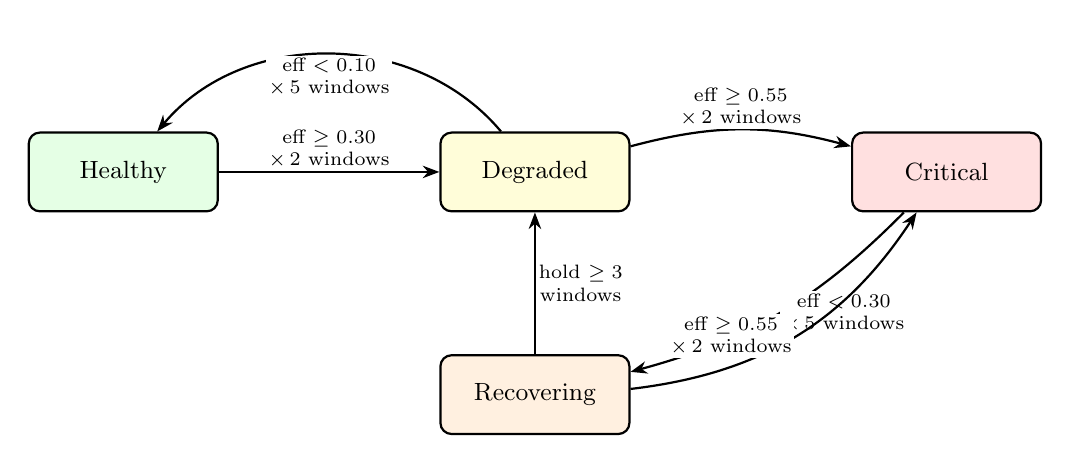
\begin{tikzpicture}[
  node distance=16mm and 28mm,
  every node/.style={font=\small},
  state/.style={rectangle, rounded corners=4pt, draw, thick, minimum width=24mm,
                minimum height=10mm, align=center},
  edge label/.style={font=\scriptsize, midway, align=center, fill=white,
                     inner sep=1pt}
]
  \node[state, fill=green!10] (H) {Healthy};
  \node[state, fill=yellow!15, right=of H] (D) {Degraded};
  \node[state, fill=red!12, right=of D] (C) {Critical};
  \node[state, fill=orange!12, below=18mm of D] (R) {Recovering};

  \draw[-{Stealth[length=6pt]}, thick]
    (H) -- node[edge label, above]{eff $\geq 0.30$\\$\times\,2$ windows} (D);
  \draw[-{Stealth[length=6pt]}, thick, bend left=15]
    (D) to node[edge label, above]{eff $\geq 0.55$\\$\times\,2$ windows} (C);
  \draw[-{Stealth[length=6pt]}, thick, bend left=15]
    (C) to node[edge label, right]{eff $< 0.30$\\$\times\,5$ windows} (R);
  \draw[-{Stealth[length=6pt]}, thick]
    (R) -- node[edge label, right]{hold $\geq 3$\\windows} (D);
  \draw[-{Stealth[length=6pt]}, thick, bend right=25]
    (R) to node[edge label, left]{eff $\geq 0.55$\\$\times\,2$ windows} (C);
  \draw[-{Stealth[length=6pt]}, thick, bend right=50]
    (D) to node[edge label, below]{eff $< 0.10$\\$\times\,5$ windows} (H);
\end{tikzpicture}
\end{center}

There is no direct path from Critical to Healthy or from Critical to
Degraded. Recovery \emph{always} passes through Recovering.

\subsection{Worked example: 20\% packet loss, then recovery}
\label{sec:walkthrough}

This walkthrough traces the engine's behavior window-by-window. Assume 3\,s
windows, default config, and an InfiniBand device with active RDMA traffic.

\begin{center}
\small
\begin{tabular}{r@{\hspace{6pt}}l@{\hspace{6pt}}c@{\hspace{6pt}}c@{\hspace{6pt}}c@{\hspace{6pt}}l}
\toprule
Win & Event & Raw & Peak & Effective & State \\
\midrule
1  & Cable fault begins. Symbol errors spike.      & 0.58 & 0.58 & 0.58 & Healthy (esc=1) \\
2  & Errors continue, link\_error\_recovery fires. & 0.60 & 0.60 & 0.60 & \textbf{Degraded} (esc=1) \\
3  & RDMA backoff: no traffic.                    & 0.54 & 0.54 & 0.54 & Degraded (esc=0) \\
4  & Traffic resumes with errors.                 & 0.58 & 0.58 & 0.58 & \textbf{Critical} (esc=2) \\
5  & Operator replaces cable. Clean traffic.       & 0.00 & 0.49 & 0.49 & Critical (stab=0) \\
6  & Clean traffic.                               & 0.00 & 0.42 & 0.42 & Critical (stab=0) \\
7  & Clean traffic.                               & 0.00 & 0.36 & 0.36 & Critical (stab=0) \\
8  & Clean traffic.                               & 0.00 & 0.30 & 0.30 & Critical (stab=0) \\
9  & Clean traffic.                               & 0.00 & 0.26 & 0.26 & Critical (stab=1) \\
10 & Clean traffic.                               & 0.00 & 0.22 & 0.22 & Critical (stab=2) \\
11 & Clean traffic.                               & 0.00 & 0.18 & 0.18 & Critical (stab=3) \\
12 & Clean traffic.                               & 0.00 & 0.16 & 0.16 & Critical (stab=4) \\
13 & Clean traffic.                               & 0.00 & 0.13 & 0.13 & \textbf{Recovering} (hold=1) \\
14 & Clean traffic.                               & 0.00 & 0.11 & 0.11 & Recovering (hold=2) \\
15 & Clean traffic.                               & 0.00 & 0.10 & 0.10 & \textbf{Degraded} (hold$\geq$3) \\
16--20 & Clean traffic. Effective decays below 0.10. & 0.00 & $<$0.10 & $<$0.10 & Degraded (stab 1..5) \\
21 & Five consecutive $< 0.10$.                   & 0.00 & 0.05 & 0.05 & \textbf{Healthy} \\
\bottomrule
\end{tabular}
\end{center}

\paragraph{Key observations.}
\begin{itemize}[nosep]
  \item Escalation to Critical took $\sim$4 windows ($\sim$12\,s).
  \item Recovery from Critical to Healthy took $\sim$17 windows ($\sim$51\,s)
        of perfectly clean input.
  \item The peak-hold track is what kept the effective score above 0.30 for
        windows 5--8 even though raw was 0.00. Without it, the engine would
        have exited Critical after just 5 clean windows.
\end{itemize}


% ============================================================================
\section{Detection Rules}
\label{sec:rules}
% ============================================================================

\subsection{Overview}

The detection engine runs 11 rules. Each examines the per-window
\texttt{AggregatedMetrics} and optionally returns an \texttt{Alert} with a
severity (\texttt{Degraded} or \texttt{Critical}).

Rules serve two purposes:
\begin{enumerate}[nosep]
  \item They produce human-readable alerts (``what is wrong?'').
  \item Their worst severity drives the coverage-weighted floor in the
        composite score (``how bad is it?'').
\end{enumerate}

Rules that depend on fabric signals declare which capabilities they consult.
Rules operating only on host-level signals (IRQ, NAPI, slab) consult no
capabilities and always receive full coverage weight.

\subsection{Rule reference}

\begin{table}[h]
\small
\begin{tabularx}{\textwidth}{p{3.6cm}cX}
\toprule
Rule name & Caps & When it fires and at what severity \\
\midrule
\texttt{InterruptAffinitySkew} & --- & Dominant CPU pct $\geq \max(70, 100/n + 45)$. Degraded; Critical if $\geq 90$\%. Needs $\geq 10$ IRQs ($\geq 1000$ on $\leq$2-CPU). \\[4pt]
\texttt{RdmaLatencySpike} & CL & Avg CQ latency $\geq 5\times$ baseline (2\,$\mu$s). Needs $\geq 10$ completions. Critical at $\geq 10\times$. \textit{Only fires in mock/replay mode.} \\[4pt]
\texttt{RdmaLinkDegradation} & LE, RS & \textit{Stateful, 5-layer.} See Section~\ref{sec:link-deg} for detailed explanation. \\[4pt]
\texttt{SlabPressure} & --- & $\geq 5000$ slab allocs \emph{and} IB errors $> 0$. Correlation detector. Critical at $> 100$ errors. \\[4pt]
\texttt{RisingErrorTrend} & LE & Total errors monotonically increasing for $\geq 3$ windows. Critical at $\geq 6$. \\[4pt]
\texttt{LatencyDrift} & CL & Slab alloc latency z-score $\geq 3$ vs EWMA baseline. Always Degraded. \\[4pt]
\texttt{ThroughputDrop} & TH & IB throughput drops $\geq 50$\% below EWMA baseline (floor-clamped at $0.5\times$ initial). Critical at $\geq 80$\%. \\[4pt]
\texttt{NapiSaturation} & --- & Avg NAPI work/budget $\geq 85$\%. Critical at $\geq 95$\%. \\[4pt]
\texttt{CqJitter} & CL & Any stall ($>50\,\mu$s completion). Immediate alert. Critical if $>10$ stalls or max $>1$\,ms. Also: p99 anomaly via z-score. \\[4pt]
\texttt{CongestionSpread} & PP, CS & \texttt{xmit\_wait} z-score $\geq 3$ \emph{and} no local hard errors. Detects upstream congestion (``victim node''). Critical at $z \geq 6$. \\[4pt]
\texttt{PcieBottleneck} & --- & CQ stalls $\geq 5$ \emph{and} slab $\geq 1000$ \emph{and} no IB errors. Always Degraded. \\
\bottomrule
\end{tabularx}
\caption{Detection rules. Capabilities: CL = CompletionLatency, LE = LinkErrors,
RS = RetransmitSignal, TH = Throughput, PP = PfcPause, CS = CreditStall.}
\label{tab:rules}
\end{table}

\subsection{Rule detail: InterruptAffinitySkew}

Detects uneven IRQ distribution across CPUs. On modern systems with RSS
(Receive Side Scaling) and \texttt{irqbalance}, interrupts should be
spread across cores. A single CPU handling a disproportionate share
indicates a misconfiguration or a saturated interrupt coalescing path.

\paragraph{Guard conditions.}
The rule is silenced when interrupt volume is too low to be meaningful:
$<10$ total IRQs per window (general), or $<1000$ on systems with $\leq 2$
CPUs (where imbalance is structurally unavoidable).

\paragraph{Effective threshold.}
The threshold adapts to CPU count:
$\text{effective} = \max(\texttt{threshold\_pct},\; 100/n_\text{cpus} + 45)$.
On a 2-CPU system this is $\max(70, 95) = 95$\%, making the rule
near-impossible to fire (by design---imbalance is expected with 2 CPUs).

\subsection{Rule detail: LatencyDrift}

Detects anomalous slab allocation latency relative to the node's own
baseline. Uses a \texttt{RollingStats} EWMA tracker ($\alpha = 0.1$) to
establish what is ``normal'' for this specific system, then fires when the
current window's average deviates by $\geq 3$ standard deviations.

\paragraph{Guard conditions.}
Requires slab latency $\geq 1000$\,ns (filters out the common case of
sub-microsecond allocations on idle systems). Also requires
\texttt{has\_network\_signal}---at least one of: IB hard errors, IB soft
errors, \texttt{rdma\_metrics.error\_count} $>0$, or
\texttt{cq\_jitter.stall\_count} $>0$. This makes it a
\textbf{correlation detector}: slab latency anomalies alone do not trigger
alerts; they must co-occur with network-layer indicators.

\paragraph{Severity.}
Always \texttt{Degraded} (never \texttt{Critical}). This reflects that slab
latency is a correlating signal, not a root cause.

\subsection{Rule detail: ThroughputDrop}

Monitors IB throughput (bytes or packets, whichever is available) via a
\texttt{RollingStats} tracker with a floor clamp. The tracker uses
$\alpha = 0.1$ and prevents the EWMA from dropping below $0.5\times$ the
initial baseline. This means a legitimate workload reduction eventually
stops triggering, but a sudden drop always fires.

\paragraph{Thresholds.}
\begin{itemize}[nosep]
  \item $\geq 50$\% drop from EWMA baseline: \texttt{Degraded}
  \item $\geq 80$\% drop: \texttt{Critical}
\end{itemize}

\subsection{Rule detail: CqJitter}

Two independent detection paths:

\begin{enumerate}[nosep]
  \item \textbf{Stall detector}: If \texttt{cq\_jitter.stall\_count} $> 0$
    (any completion $> 50\,\mu$s), fire immediately. Escalate to
    \texttt{Critical} if $> 10$ stalls or max latency $> 1$\,ms.
  \item \textbf{p99 anomaly}: Uses a \texttt{RollingStats} tracker with
    clamp $[0.1, 5.0]$ on the estimated p99 latency. After warmup, fires
    \texttt{Degraded} if z-score $\geq 3$.
\end{enumerate}

\subsection{Rule detail: CongestionSpread}

Detects upstream fabric congestion affecting this node as a ``victim.''
The key insight: when a remote node or switch is congested, IB flow control
causes \texttt{port\_xmit\_wait} to rise on the local port---but the local
node has no hard errors of its own.

\paragraph{Guard conditions.}
Requires: (i) warmup complete, (ii) $\texttt{xmit\_wait} \geq 1$, (iii)
$\texttt{total\_hard\_error\_delta} + \texttt{link\_error\_recovery\_delta}
= 0$ (no local errors), (iv) z-score $\geq 3$.

\paragraph{Why exclude local errors.}
If the node has its own hard errors, the signal is likely a local problem,
not upstream congestion. The rule only fires when the node itself is clean
but being starved by its neighbors.

\subsection{Rule detail: PcieBottleneck}

A heuristic detector for PCIe bus saturation. Fires when CQ stalls
($\geq 5$) and slab pressure ($\geq 1000$ allocs) co-occur \emph{without}
any IB errors. The logic: if completions are stalling and memory allocation
is pressured, but the IB link is healthy, the bottleneck is likely between
the NIC and CPU (PCIe).

Always \texttt{Degraded}---never \texttt{Critical}---because this is an
indirect inference, not a direct observation.

\subsection{Deep dive: RdmaLinkDegradation (the most complex rule)}
\label{sec:link-deg}

This rule models the real-world failure sequence for an InfiniBand cable:
\textit{Nominal $\rightarrow$ Elevated Errors $\rightarrow$ Link Recovery
$\rightarrow$ Link Down.} It is stateful, maintains three
\texttt{RollingStats} trackers (symbol errors, receive errors, soft errors),
an \texttt{elevated\_windows} counter (capped at 10), and a cooldown timer.
It uses five detection layers, checked in priority order from most severe to
least:

\begin{enumerate}
  \item \textbf{Link downed} ($\texttt{link\_downed\_delta} > 0$):
        Immediately Critical. The cable is dead; replace it.
  \item \textbf{Link recovery} ($\texttt{link\_error\_recovery\_delta} > 0$):
        Immediately Critical. The firmware is actively trying to recover a
        failing link. This event precedes link-down and is the earliest
        warning of a dying cable.
  \item \textbf{Error budget exceeded}
        ($\texttt{total\_hard\_error\_delta} > \texttt{error\_budget}$,
        default 5 per window):
        Degraded, or Critical if $> 10\times$ budget (50). The budget is a
        per-window count, not a rate---this fires even at low throughput.
  \item \textbf{Absolute error rate ceiling} ($\geq 5$\%):
        On links with traffic, if
        $\texttt{total\_all\_errors\_delta()} / \texttt{throughput} \geq 0.05$
        fires unconditionally. This catches sustained degradation that the
        EWMA might adapt to (the ``boiling frog'' scenario). On Soft-RoCE
        devices, uses soft-error totals instead.
  \item \textbf{Rate anomaly via z-score} ($z \geq 3$ after warmup):
        Computes $z = \max(z_\text{sym}, z_\text{rcv}, z_\text{soft})$
        using clamped EWMA trackers. Requires $\texttt{total\_errors} > 0$.
        Critical at $z \geq 2\times\texttt{threshold}$ (6), or after
        $\geq 3$ consecutive elevated windows, or if the total error rate
        $\geq 3\times$ the absolute ceiling ($15$\%).
\end{enumerate}

\paragraph{State management.}
When any layer fires, \texttt{elevated\_windows} increments (capped at 10)
and \texttt{cooldown\_remaining} resets to 3. When no layer fires and
cooldown is active, \texttt{cooldown\_remaining} decrements. When cooldown
expires, \texttt{elevated\_windows} decrements (step-down). This provides
a memory of recent degradation that decays gradually.

\paragraph{The ``boiling frog'' defense.}
Rules that use EWMA baselines have a risk: if an error rate rises slowly
enough, the EWMA adapts to it and the z-score stays low. The
\texttt{RollingStats} tracker addresses this with \emph{clamping}: after
a 5-window warmup, it captures the EWMA as a baseline and prevents the
EWMA from drifting above $3\times$ baseline. This means a slowly rising
error rate will eventually exceed the clamped EWMA and trigger an anomaly.

The absolute error rate ceiling (layer 4) provides a second defense:
regardless of what the EWMA thinks is ``normal,'' any window with
$\geq 5$\% error rate fires unconditionally.

\subsection{RollingStats: the statistical backbone}
\label{sec:rolling-stats}

Several rules (\texttt{RdmaLinkDegradation}, \texttt{LatencyDrift},
\texttt{ThroughputDrop}, \texttt{CqJitter}, \texttt{CongestionSpread})
depend on the \texttt{RollingStats} tracker
(\texttt{detection/rolling\_stats.rs}). Its behavior is central to
understanding why rules fire when they do.

\paragraph{EWMA update.}
On each observation $x_t$:
\[
  \text{ewma}_t = \text{ewma}_{t-1} + \alpha \cdot (x_t - \text{ewma}_{t-1})
\]
After update, the EWMA is clamped:
$\text{ewma}_t \leftarrow \min(\text{ewma}_t,\; \text{baseline} \times
\text{clamp\_hi})$, where the baseline is frozen after warmup. Without this
clamp, a gradually worsening signal would drag the EWMA upward and the
z-score would never fire.

\paragraph{Variance tracking.}
Uses an EWMA of squared deviations:
\[
  \text{var}_t = \text{var}_{t-1} + \alpha \cdot
  \left((x_t - \text{ewma}_t)^2 - \text{var}_{t-1}\right)
\]
Standard deviation: $\sigma_t = \sqrt{\text{var}_t}$.

\paragraph{Z-score.}
\[
  z_t = \frac{x_t - \text{ewma}_t}{\max(\sigma_t, \epsilon)}
\]
where $\epsilon$ is a small floor to prevent division by near-zero. A
$z \geq 3$ indicates the observation is 3+ standard deviations above the
expected value.

\paragraph{Floor clamp.}
\texttt{RollingStats::with\_floor($\alpha$, floor\_factor)} prevents the
EWMA from dropping below $\texttt{floor\_factor} \times \text{initial}$.
Used by \texttt{ThroughputDrop} with floor 0.5: if throughput drops to
30\% of baseline, the EWMA stops at 50\%, making the z-score reflect the
full gap. Without the floor, a gradual workload ramp-down would drag the
EWMA down and mask a genuine drop.

\paragraph{TrendTracker.}
A companion type that tracks \emph{monotonically increasing} sequences.
Each window, if $x_t > x_{t-1}$, \texttt{consecutive\_increases}
increments; otherwise it resets. Used by \texttt{RisingErrorTrendRule}
to detect sustained degradation trajectories.


% ============================================================================
\section{Multi-Timescale Evaluation and Burst Classification}
\label{sec:timescale}
% ============================================================================

\subsection{Why multiple timescales?}

A single smoother with $\alpha = 0.3$ responds in a few windows. This is
good for detecting sudden faults but blind to slow, multi-minute drift.
Conversely, a slow smoother ($\alpha = 0.1$) catches drift but ignores brief
bursts.

The engine solves this by running three parallel
\texttt{SmoothedHealthScore} + \texttt{HealthStateMachine} pairs, each with
different parameters:

\begin{center}
\begin{tabular}{lcccc}
\toprule
Track & EWMA $\alpha$ & Peak decay $\rho$ & Enter dwell & Exit dwell \\
\midrule
Fast   & 0.6 & 0.5  & 1 & 2--3 \\
Medium & 0.3 & 0.85 & 2 & 5 \\
Slow   & 0.1 & 0.95 & 4 & 8--10 \\
\bottomrule
\end{tabular}
\end{center}

The composite verdict across the three tracks is the \textbf{worst observed
state}.

\begin{warningbox}
  \textbf{Important caveat:} the multi-timescale evaluator is currently
  published for telemetry and consumed by the burst classifier, but it does
  \textbf{not} drive the authoritative health state. The single-track Medium
  state machine alone governs \texttt{current\_state()} and the scheduler.
  This means operators can see \texttt{Critical} on the fast track in Grafana
  while the official state is \texttt{Degraded}.
\end{warningbox}

\subsection{Burst classification}

The \texttt{BurstClassifier} (\texttt{detection/burst.rs}) uses a sliding
window of 30 recent evaluations. Any window where the raw score $\geq 0.40$
counts as a ``burst event.'' The classifier then cross-references the
timescale states:

\begin{center}
\begin{tabular}{lcp{7cm}}
\toprule
Classification & Condition & Meaning \\
\midrule
\texttt{Quiet}              & No bursts, slow track Healthy & Normal operation. \\
\texttt{Burst}              & Bursts detected, slow track Healthy & Short spikes---probably transient. \\
\texttt{Sustained}          & No bursts, slow track Degraded/Critical & Slow drift without sharp peaks. \\
\texttt{MixedBurstSustained}& Bursts + slow track Degraded/Critical & Both burst and drift occurring. \\
\bottomrule
\end{tabular}
\end{center}

This classification is exposed via the
\texttt{argus\_burst\_classification} Prometheus gauge and is intended for
use by the scheduler to differentiate responses (e.g., a burst warrants
caution but not immediate drain).

% ============================================================================
\section{Timing Model}
\label{sec:timing}
% ============================================================================

\subsection{Time constants at a glance}

With the default 3\,s window, the real-world time for each transition:

\begin{center}
\begin{tabular}{lcc}
\toprule
Transition & Min windows & Wall-clock time \\
\midrule
Healthy $\rightarrow$ Degraded & 2 & $\sim$6\,s \\
Degraded $\rightarrow$ Critical & 2 & $\sim$6\,s \\
Critical $\rightarrow$ Recovering & 5 + peak-hold decay & $\sim$27\,s \\
Recovering $\rightarrow$ Degraded & 3 & $\sim$9\,s \\
Degraded $\rightarrow$ Healthy & 5 & $\sim$15\,s \\
\midrule
\textbf{Healthy $\rightarrow$ Critical (min)} & \textbf{4} & $\mathbf{\sim}$\textbf{12\,s} \\
\textbf{Critical $\rightarrow$ Healthy (min)} & \textbf{$\sim$18} & $\mathbf{\sim}$\textbf{54\,s} \\
\bottomrule
\end{tabular}
\end{center}

\paragraph{Note on peak-hold.}
The ``Critical $\rightarrow$ Recovering'' transition requires not just 5
windows of $\text{effective} < 0.30$, but 5 consecutive windows where the
peak-hold track has decayed below 0.30. From a peak of 0.6, this decay
alone takes 5 windows ($0.6 \times 0.85^5 = 0.27$). Combining peak-hold
decay and dwell requirements, at least $\sim$9 windows elapse before
reaching Recovering.

\subsection{Timing edge cases}

\paragraph{Window boundary jitter.}
The tick loop sleeps 200\,ms between checks. Actual window duration varies
between $[3.0, 3.2]$\,s. Over many windows, this jitter is
inconsequential---but it means transitions can take one tick longer than
the minimum.

\paragraph{Capability provider latency.}
Providers run sequentially within \texttt{collect\_all}. There is no
per-provider timeout. A slow sysfs read extends the evaluation phase,
potentially skewing the next window boundary.


% ============================================================================
\section{Failure Modes}
\label{sec:failure-modes}
% ============================================================================

This section documents known limitations and surprising behaviors, each tied
to specific implementation details.

\subsection{Recovery takes longer than expected}

\paragraph{Root cause.}
The peak-hold decay, the 5-window dwell for exiting Critical, the 3-window
hold in Recovering, and another 5-window dwell for exiting Degraded combine
to require $\sim$18 windows ($\sim$54\,s) of clean input to return to Healthy
from Critical. This is intentional---verified by the test
\texttt{full\_recovery\_path\_critical\_to\_healthy}.

\paragraph{Operator impact.}
An operator who removes a fault (e.g., by deleting a \texttt{tc netem}
rule) will see the node remain in Critical/Recovering/Degraded for roughly
one minute.

\subsection{Carry-forward extends recovery when workload stops}

\paragraph{Root cause.}
If the RDMA workload stops entirely (no traffic, no errors), the carry-forward
mechanism (Section~\ref{sec:carry-forward}) keeps the raw score elevated at
$0.9^k$ of its previous value. From $0.6$, this takes 7 windows ($\sim$21\,s)
to decay below $0.30$.

\paragraph{Operator impact.}
Draining the workload as a remediation does not immediately signal recovery.

\subsection{Missing or incomplete sysfs counter layout}

\paragraph{Root cause.}
Not all RDMA devices expose the same sysfs counters. On real IB HCAs, the
standard \texttt{counters/} directory provides byte-level throughput
(\texttt{port\_rcv\_data}, \texttt{port\_xmit\_data}) and all hard-error
counters---the engine operates at full fidelity. On software RDMA devices
(RXE/Soft-RoCE) that expose only \texttt{hw\_counters/},
\texttt{throughput\_bytes()} returns 0 and the engine falls back to
\texttt{throughput\_pkts()}. If neither byte nor packet counters are
available, \texttt{has\_traffic()} returns false and the soft-error score
term contributes nothing.

\paragraph{Operator impact.}
On devices with incomplete counter layouts, the engine is under-sensitive to
RDMA-specific faults. The score is driven only by IRQ, slab, NAPI, and CQ
jitter signals. This primarily affects Soft-RoCE test environments; real IB
deployments are unaffected.

\subsection{Capability fusion never reduces the score}

\paragraph{Root cause.}
The fusion contribution is $\geq 0$ by construction. A capability provider
that reports ``no problems'' contributes $\Delta = 0$, not a negative value.

\paragraph{Operator impact.}
If a rule fires based on partial data and the capability providers have
better data showing the node is healthy, the providers cannot override the
rule. The only attenuation path is the coverage-weighted floor
(Section~\ref{sec:coverage-floor}), which requires the consulted capabilities
to be \texttt{Absent}.

\subsection{Determinism with caveats}

The engine itself is deterministic: the test
\texttt{state\_machine\_is\_deterministic} verifies that the same raw-score
sequence always produces the same state sequence. However, inputs are
non-deterministic: sysfs reads and BPF map reads happen on the agent thread
without synchronization with the kernel, and 200\,ms tick jitter determines
which observations land in which window.


% ============================================================================
\section{Observability and Debuggability}
\label{sec:observability}
% ============================================================================

\subsection{What is exported}

The agent exposes the following via Prometheus (\texttt{/metrics}) and JSON
endpoints:

\paragraph{Health state and score.}
\texttt{argus\_health\_state} (0/1/2/3 for H/D/C/R),
\texttt{argus\_health\_score\_millis},
\texttt{argus\_health\_score\_raw\_millis},
\texttt{argus\_health\_score\_ewma\_millis},
\texttt{argus\_health\_score\_peak\_hold\_millis},
\texttt{argus\_health\_score\_effective\_millis}.

\paragraph{Capability layer.}
\texttt{argus\_capability\_coverage\{capability,quality\}},
\texttt{argus\_capability\_grade},
\texttt{argus\_sample\_contribution\_millis}.

\paragraph{Multi-timescale.}
\texttt{argus\_timescale\_state\{timescale\}},
\texttt{argus\_timescale\_score\_millis\{timescale\}}.

\paragraph{Alerts and transitions.}
\texttt{argus\_alert\_count\{kind,severity\}},
\texttt{argus\_state\_transitions\{from,to\}}.

\paragraph{HTTP endpoints.}
\texttt{/metrics} (Prometheus), \texttt{/health} (state JSON),
\texttt{/status} (full JSON with recent alerts), \texttt{/coverage}
(capability coverage report).

\paragraph{Structured logs.}
\texttt{tracing::info!} on every state transition (with \texttt{from},
\texttt{to}, \texttt{seq}) and on capability tier selection at startup.
\texttt{tracing::warn!} on the stuck-state watchdog (200 windows in one
state).

\subsection{What is not exported}

\begin{itemize}[nosep]
  \item \textbf{Per-rule firing rate.} There is no ``rule X fired 8 of the
        last 10 windows'' metric.
  \item \textbf{Carry-forward indicator.} An operator cannot tell from
        exported data whether a high score comes from fresh signal or
        carry-forward. The \texttt{prev\_raw\_score} field is internal.
  \item \textbf{Rule evidence.} \texttt{RuleEvidence} is defined in
        \texttt{fusion.rs} but not emitted on the \texttt{Alert} struct.
  \item \textbf{Link degradation rule internals.} The
        \texttt{elevated\_windows}, \texttt{cooldown\_remaining}, and
        \texttt{link\_state} fields of \texttt{RdmaLinkDegradationRule}
        are not surfaced.
\end{itemize}

\subsection{How to trace a decision}

When a node is in an unexpected state, follow these steps:

\begin{enumerate}
  \item \textbf{Read \texttt{/status}.} Contains the full
        \texttt{AggregatedMetrics} and the last 100 alerts.
  \item \textbf{Compare raw vs.\ peak\_hold.} If
        \texttt{peak\_hold\_millis} $\gg$ \texttt{raw\_millis}, the engine
        is in residual hold from a past spike. The node will stay in its
        current state until peak decays below the exit threshold.
  \item \textbf{Check \texttt{/coverage}.} If a rule's consulted capability
        is \texttt{Absent}, the coverage-weighted floor for that rule is 0;
        the rule's verdict alone cannot push the score up.
  \item \textbf{Compare timescale states.} If the fast track says
        \texttt{Critical} and the slow track says \texttt{Healthy}, the
        problem is a short burst. If the slow track also says
        \texttt{Critical}, it is a sustained problem.
  \item \textbf{Check \texttt{state\_transitions\{from,to\}}.} Persistent
        flap (many transitions) is evidence of an oscillating \emph{input},
        not an engine bug. The default config makes flap from clean windows
        impossible (verified by tests).
\end{enumerate}


% ============================================================================
\section{Limitations and Gaps}
\label{sec:limitations}
% ============================================================================

\subsection{Signals the engine cannot observe today}

\begin{description}[style=nextline,leftmargin=0.5cm]
  \item[CQ latency via eBPF.]
    \texttt{RdmaLatencySpikeRule} reads \texttt{rdma\_metrics}, populated
    only in mock/replay mode. Live eBPF kprobes currently attach to
    RXE-specific symbols (\texttt{rxe\_post\_send}/\texttt{rxe\_poll\_cq}).
    On production IB hardware (\texttt{mlx5}, \texttt{hfi1}), these symbols
    do not exist and the rule is inert. Vendor-specific kprobe targets for
    \texttt{mlx5} CQ completion paths have not yet been added.
  \item[PCIe link-state changes.]
    \texttt{PcieBottleneckRule} infers PCIe pressure indirectly (CQ stalls
    + slab pressure $-$ IB errors). It cannot observe PCIe AER events.
  \item[Counter wraparound.]
    32-bit IB counters are handled via \texttt{saturating\_sub}. A wrap
    produces delta = 0 for one window (under-detection), then normal deltas
    resume.
  \item[Asymmetric faults.]
    The engine has no concept of ``the remote end caused this.'' A receiver
    node experiencing degradation from a bad remote sender may not produce
    local signals. Cross-node correlation is external.
\end{description}

\subsection{Assumption failures}

\begin{description}[style=nextline,leftmargin=0.5cm]
  \item[Devices with incomplete sysfs counters.]
    On devices (primarily Soft-RoCE/RXE) where neither byte nor packet
    throughput counters are available, \texttt{has\_traffic()} is false and
    the soft-error term is silenced. Real IB HCAs expose the standard
    \texttt{counters/} directory and are not affected.
  \item[2-CPU systems.]
    The IRQ skew effective threshold reaches 95\% ($100/2 + 45$), making
    it nearly impossible to trigger the IRQ skew score term.
  \item[Throughput floor.]
    The $0.5\times$ floor on \texttt{ThroughputDropRule} means a legitimate
    workload reduction to 30\% of baseline registers as a ``drop'' until the
    window passes.
\end{description}

\subsection{Missing safeguards}

\begin{itemize}[nosep]
  \item The stuck-state watchdog (200 windows) only logs; it does not
        auto-reset.
  \item No per-provider timeout in capability collection.
  \item No torn-read detection for sysfs counters.
  \item No 32-bit counter wrap detection.
\end{itemize}


% ============================================================================
\section{Summary of Actual Behavior}
\label{sec:summary}
% ============================================================================

This section describes what the engine actually does under specific
scenarios---no generalization, just observable behavior.

\paragraph{Degrading IB cable with rising symbol errors.}
On a real IB fabric, a failing cable produces \texttt{symbol\_error} and
\texttt{link\_error\_recovery} deltas. \texttt{link\_error\_recovery} $> 0$
adds 0.35 to the composite score immediately, and
\texttt{RdmaLinkDegradation} fires at Critical severity. The
coverage-weighted floor pushes raw to $\geq 0.55$. State reaches Critical
after 2--4 windows ($\sim$6--12\,s). Remains Critical until errors stop
for $\sim$54\,s.

\paragraph{Sustained packet loss on Soft-RoCE.}
Soft-error rate $\geq 5$\% triggers \texttt{RdmaLinkDegradation}'s absolute
ceiling every window. The composite raw score reaches $\sim$0.55+ via the
soft-error term plus the coverage-weighted severity floor. Behavior is
otherwise identical to the IB case above.

\paragraph{Brief spike (5 windows) then perfect quiet.}
State reaches Critical after 4 windows of evidence. After the spike ends,
peak-hold keeps effective score above \texttt{critical\_exit} for $\sim$5
windows. Total time from spike end to Healthy: $\sim$17 additional windows
($\sim$51\,s).

\paragraph{Slow drift over 10 minutes.}
\texttt{RdmaLinkDegradation}'s clamped EWMA prevents adaptation. The absolute
ceiling fires once the rate exceeds 5\%. \texttt{RisingErrorTrendRule} fires
after 3 monotonically increasing windows.

\paragraph{Healthy node adjacent to a failing cable.}
No local hard errors. \texttt{port\_xmit\_wait} may rise due to upstream
credit stalls. \texttt{CongestionSpreadRule} fires when z-score $\geq 3$.
The composite score receives a 0.10 ``victim buffer'' boost.

\paragraph{Workload stops (no traffic, no errors).}
Carry-forward decays raw at $0.9\times$/window. Score decreases over $\sim$7
windows. State machine de-escalates on the smoothed schedule.

\paragraph{All fabric capabilities are \texttt{Absent}.}
Rules still fire and emit alerts, but the coverage-weighted floor is zero.
The raw score depends entirely on the \texttt{compute\_health\_score}
formula. Detection is reduced but not eliminated.


% ============================================================================
\section{eBPF Kernel Probes}
\label{sec:ebpf}
% ============================================================================

This section documents the in-kernel instrumentation that produces the raw
data the detection engine evaluates.

\subsection{Probe programs}

The eBPF object (\texttt{argus-ebpf/src/}) contains four source files, each
implementing probes for a specific subsystem:

\begin{table}[h]
\centering
\small
\begin{tabularx}{\textwidth}{p{3.4cm}p{3.8cm}X}
\toprule
File & Programs & Kernel attachment \\
\midrule
\texttt{slab.rs} & \texttt{trace\_kmem\_cache\_alloc}, \texttt{trace\_kmem\_cache\_free}, \texttt{kprobe\_slab\_alloc\_entry}, \texttt{kretprobe\_slab\_alloc} & Tracepoints \texttt{kmem/kmem\_cache\_alloc}, \texttt{kmem/kmem\_cache\_free}; kprobe/kretprobe on \texttt{kmem\_cache\_alloc} \\[4pt]
\texttt{interrupts.rs} & \texttt{trace\_irq\_handler\_entry}, \texttt{trace\_napi\_poll} & Tracepoints \texttt{irq/irq\_handler\_entry}, \texttt{napi/napi\_poll} \\[4pt]
\texttt{rdma\_jitter.rs} & \texttt{kprobe\_wr\_submit}, \texttt{kprobe\_cq\_poll\_entry}, \texttt{kretprobe\_cq\_poll} & Kprobes resolved from \texttt{/proc/kallsyms} at runtime \\
\bottomrule
\end{tabularx}
\caption{eBPF probe programs and their kernel attachments.}
\end{table}

\subsection{BPF maps}

All data flows from kernel to userspace through per-CPU array maps (no ring
buffer for the hot path). This keeps probe overhead under 5\,$\mu$s.

\begin{table}[h]
\centering
\small
\begin{tabularx}{\textwidth}{p{3.5cm}p{3cm}X}
\toprule
Map name & Type & Contents \\
\midrule
\texttt{IRQ\_COUNTS} & PerCpuArray\texttt{<u64>} & 1 slot per CPU: cumulative IRQ handler entry count \\[2pt]
\texttt{SLAB\_STATS} & PerCpuArray\texttt{<[u64;6]>} & \texttt{[alloc\_count, free\_count, total\_bytes\_req, total\_bytes\_alloc, total\_latency\_ns, max\_latency\_ns]} \\[2pt]
\texttt{SLAB\_ALLOC\_SCRATCH} & LruHashMap\texttt{<u64,u64>} & Key: \texttt{pid\_tgid}; value: entry timestamp for latency pairing. Max 256 entries. \\[2pt]
\texttt{NAPI\_STATS} & PerCpuArray\texttt{<[u64;3]>} & \texttt{[poll\_count, total\_work, total\_budget]} \\[2pt]
\texttt{WR\_TIMESTAMPS} & LruHashMap\texttt{<u64,u64>} & Key: QP number; value: WR submit timestamp. Max 4096 entries. \\[2pt]
\texttt{CQ\_JITTER\_STATS} & PerCpuArray\texttt{<[u64;4]>} & \texttt{[completion\_count, total\_latency\_ns, max\_latency\_ns, stall\_count]} where stall threshold = 50\,$\mu$s \\[2pt]
\texttt{QP\_OWNERS} & LruHashMap\texttt{<u32,u32>} & QP $\rightarrow$ TGID. Max 4096 entries. \\[2pt]
\texttt{CQ\_POLL\_SCRATCH} & LruHashMap\texttt{<u64,u64>} & Key: \texttt{pid\_tgid}; value: \texttt{wc} pointer. Max 256 entries. \\[2pt]
\texttt{LRU\_MISSES} & PerCpuArray\texttt{<[u64;2]>} & \texttt{[cq\_lru\_misses, slab\_lru\_misses]}. Counts when LRU lookup fails (eviction indicator). \\[2pt]
\texttt{OFFSETS} & Array\texttt{<u32>} & 8 entries: tracepoint field offsets and BTF struct offsets populated by userspace at load time. \\
\bottomrule
\end{tabularx}
\caption{All BPF maps declared in \texttt{argus-ebpf/src/main.rs}.}
\end{table}

\subsection{CQ jitter measurement path}

The CQ latency measurement works by correlating work request (WR) submission
timestamps with completion queue (CQ) poll return values:

\begin{enumerate}[nosep]
  \item \textbf{WR submit kprobe}: Reads \texttt{qp\_num} from the
        \texttt{ib\_qp} struct (using BTF offsets from \texttt{OFFSETS}),
        stores \texttt{(qp\_num $\rightarrow$ ktime\_ns)} in
        \texttt{WR\_TIMESTAMPS} and \texttt{(qp\_num $\rightarrow$ pid)} in
        \texttt{QP\_OWNERS}.
  \item \textbf{CQ poll entry kprobe}: Saves the \texttt{ib\_wc} pointer
        in \texttt{CQ\_POLL\_SCRATCH}.
  \item \textbf{CQ poll kretprobe}: Iterates up to
        $\min(\texttt{num\_completions}, 8)$ completions with stride 80 bytes.
        For each, reads \texttt{wc[i].qp $\rightarrow$ qp\_num}, looks up
        the submit timestamp in \texttt{WR\_TIMESTAMPS}, computes
        $\texttt{latency} = \texttt{now} - \texttt{submit\_ts}$, and updates
        \texttt{CQ\_JITTER\_STATS}. If the WR timestamp lookup fails (LRU
        eviction), increments \texttt{LRU\_MISSES[0]}.
\end{enumerate}

\begin{warningbox}
  The LRU maps have fixed capacity. Under high QP counts ($>4096$ active
  queue pairs), \texttt{WR\_TIMESTAMPS} entries are evicted before CQ poll,
  causing latency measurements to be lost. The
  \texttt{argus\_ebpf\_lru\_evictions\{map=cq\}} Prometheus counter tracks
  this. If eviction rates are high, the CQ jitter metrics become unreliable.
\end{warningbox}


% ============================================================================
\section{Hardware Counter Collection}
\label{sec:hw-counters}
% ============================================================================

\subsection{Counter types}

The agent reads 17 distinct counter types from
\texttt{/sys/class/infiniband/*/ports/*/}. Each is identified by a
discriminant byte in the aggregator:

\begin{center}
\small
\begin{tabular}{clp{5.5cm}}
\toprule
ID & Counter & sysfs path suffix \\
\midrule
0  & \texttt{symbol\_error}             & \texttt{counters/symbol\_error\_count} \\
1  & \texttt{link\_downed}              & \texttt{counters/link\_downed} \\
2  & \texttt{port\_rcv\_errors}         & \texttt{counters/port\_rcv\_errors} \\
3  & \texttt{port\_xmit\_discards}      & \texttt{counters/port\_xmit\_discards} \\
4  & \texttt{port\_rcv\_data}           & \texttt{counters/port\_rcv\_data} \\
5  & \texttt{port\_xmit\_data}          & \texttt{counters/port\_xmit\_data} \\
6  & \texttt{port\_rcv\_remote\_phys}   & \texttt{counters/port\_rcv\_remote\_physical\_errors} \\
7  & \texttt{local\_link\_integrity}    & \texttt{counters/local\_link\_integrity\_errors} \\
8  & \texttt{excessive\_buffer\_overrun}& \texttt{counters/excessive\_buffer\_overrun\_errors} \\
9  & \texttt{hw\_rcv\_pkts}             & \texttt{hw\_counters/rx\_read\_requests} \\
10 & \texttt{hw\_xmit\_pkts}            & \texttt{hw\_counters/tx\_write\_requests} \\
11 & \texttt{rxe\_duplicate\_request}   & \texttt{hw\_counters/duplicate\_request} \\
12 & \texttt{rxe\_seq\_error}           & \texttt{hw\_counters/seq\_error} \\
13 & \texttt{rxe\_retry\_exceeded}      & \texttt{hw\_counters/retry\_exceeded\_err} \\
14 & \texttt{rxe\_send\_error}          & \texttt{hw\_counters/send\_err} \\
15 & \texttt{link\_error\_recovery}     & \texttt{counters/link\_error\_recovery} \\
16 & \texttt{port\_xmit\_wait}          & \texttt{counters/port\_xmit\_wait} \\
\bottomrule
\end{tabular}
\end{center}

\paragraph{Throughput note.}
IB \texttt{port\_rcv\_data} and \texttt{port\_xmit\_data} report values in
units of 4 bytes (32-bit words). The Prometheus metrics multiply by 4 to
report actual bytes: \texttt{argus\_ib\_throughput\_rcv\_bytes} $=$
\texttt{port\_rcv\_data\_delta} $\times$ $4$.

\paragraph{Delta accumulation.}
Deltas from multiple ports on the same device are summed into a single
\texttt{IbCounterDeltas} struct. This means on a dual-port HCA, error deltas
reflect the aggregate across both ports.

\subsection{Derived metrics}

The \texttt{IbCounterDeltas} struct provides several computed accessors:
\begin{itemize}[nosep]
  \item \texttt{total\_hard\_error\_delta()}: symbol + rcv errors + remote physical + link integrity + buffer overrun
  \item \texttt{total\_soft\_error\_delta()}: RXE duplicate + seq error + retry exceeded + send error
  \item \texttt{throughput\_bytes()}: $(\texttt{rcv\_data} + \texttt{xmit\_data}) \times 4$
  \item \texttt{throughput\_pkts()}: rcv + xmit packet counts
  \item \texttt{has\_traffic()}: bytes $> 0$ or pkts $> 0$
\end{itemize}


% ============================================================================
\section{Capability System}
\label{sec:capabilities}
% ============================================================================

\subsection{Design rationale}

Different RDMA hardware exposes different observability surfaces. An IB HCA
with full sysfs counters, a RoCE NIC with ethtool stats, and a Soft-RoCE
device with minimal \texttt{hw\_counters/} each require different backends
to extract the same logical signal. The capability system abstracts this:
each logical signal (e.g., ``link errors'') can have multiple backend
implementations, and the best available one is selected at startup.

\subsection{Capabilities}

Each capability represents a logical signal type:

\begin{center}
\small
\begin{tabular}{lp{8cm}}
\toprule
Capability & What it measures \\
\midrule
\texttt{LinkErrors}        & Error counters (symbol, rcv, link integrity, etc.) \\
\texttt{Throughput}        & Byte/packet throughput rate \\
\texttt{CompletionLatency} & CQ completion latency distribution (p50--p999) \\
\texttt{RetransmitSignal}  & Retransmission rate or indicators \\
\texttt{PfcPause}          & PFC (Priority Flow Control) pause frame counts \\
\texttt{CreditStall}       & IB credit stalls (\texttt{port\_xmit\_wait}) \\
\texttt{QpAttribution}     & Map QP numbers to processes \\
\texttt{PeerLiveness}      & Remote node health (probe-based) \\
\texttt{EcnSignal}         & ECN marking rates \\
\texttt{CnpSignal}         & Congestion Notification Packet rates \\
\bottomrule
\end{tabular}
\end{center}

\subsection{Quality levels and coverage grading}

Each provider declares a quality level based on how trustworthy its data is:

\begin{center}
\begin{tabular}{lcl}
\toprule
Quality & Weight & Meaning \\
\midrule
\texttt{High}   & 1.0 & Direct hardware counters \\
\texttt{Medium} & 0.6 & Derived or sampled data \\
\texttt{Low}    & 0.3 & Heuristic or inferred \\
\texttt{Absent} & 0.0 & Not available on this hardware \\
\bottomrule
\end{tabular}
\end{center}

At startup, the \texttt{CapabilityRegistry} probes all candidate providers
and selects the highest-quality available backend for each capability.
A \texttt{CoverageReport} is assembled with an overall grade:

\begin{description}[nosep]
  \item[Grade A] All four critical capabilities (\texttt{LinkErrors},
    \texttt{Throughput}, \texttt{CompletionLatency}, \texttt{RetransmitSignal})
    at \texttt{High} quality.
  \item[Grade B] All critical capabilities at \texttt{Medium} or above.
  \item[Grade C] At least one critical capability is non-\texttt{Absent}.
  \item[Grade F] All critical capabilities are \texttt{Absent} (e.g., no IB
    hardware present).
\end{description}

\subsection{Provider backends}

The system ships with 17 candidate providers:

\begin{multicols}{2}
\begin{itemize}[nosep]
  \item \texttt{SysfsLinkErrors}
  \item \texttt{InferredLinkErrors}
  \item \texttt{SysfsThroughput}
  \item \texttt{EbpfCqLatency}
  \item \texttt{ThroughputProxyLatency}
  \item \texttt{EbpfRetransmit}
  \item \texttt{MadRetransmit}
  \item \texttt{SysfsRetransmit}
  \item \texttt{InferredRetransmit}
  \item \texttt{EbpfQpAttribution}
  \item \texttt{RdmaCoreQpAttribution}
  \item \texttt{SysfsRxeQpAttribution}
  \item \texttt{EthtoolPfc}
  \item \texttt{InferredPfc}
  \item \texttt{EthtoolEcn}
  \item \texttt{EthtoolCnp}
  \item \texttt{PeerLiveness}
\end{itemize}
\end{multicols}


% ============================================================================
\section{Scheduler Integration}
\label{sec:scheduler}
% ============================================================================

\subsection{Architecture}

The scheduler subsystem bridges ARGUS health verdicts and workload
schedulers. It uses a reconciliation loop: each cycle, the reconciler
compares the \emph{desired} node state (derived from ARGUS health) against
the \emph{observed} state (queried from the scheduler backend) and takes
action to converge them.

\subsection{State model}

\begin{center}
\small
\begin{tabular}{ll}
\toprule
Desired states & Observed states \\
\midrule
\texttt{Available}       & \texttt{Available} \\
\texttt{Draining}        & \texttt{Draining} (jobs still running) \\
\texttt{HeldByOperator}  & \texttt{Drained} (empty) \\
                          & \texttt{Down} \\
                          & \texttt{Unknown} \\
\bottomrule
\end{tabular}
\end{center}

\subsection{Policy}

The \texttt{SchedulingPolicy} maps health states to desired states:

\begin{itemize}[nosep]
  \item \textbf{Healthy} $\rightarrow$ \texttt{Available} (unless operator hold is set)
  \item \textbf{Degraded / Recovering} $\rightarrow$ \texttt{Draining} only if
        \texttt{drain\_on\_degraded} is enabled; otherwise, keeps current desired state
  \item \textbf{Critical} $\rightarrow$ \texttt{Draining} always
\end{itemize}

Operator holds (\texttt{HeldByOperator}) are never auto-cleared. They
require explicit release via \texttt{/scheduler/release} or the
\texttt{argus-scheduler release} CLI.

\subsection{Safety mechanisms}

\begin{description}[style=nextline,leftmargin=0.5cm]
  \item[Advisory lock]
    The reconciler holds an \texttt{flock} on
    \texttt{/var/run/argus/scheduler.lock} to prevent concurrent
    reconciliation from multiple agent instances.
  \item[Drain rate limit]
    Default maximum 3 drains per hour. Rejections are counted in
    \texttt{argus\_scheduler\_drain\_rejected\_total}.
  \item[Resume cooldown]
    Default 60 seconds after drain before a resume is allowed.
  \item[Contested resume detection]
    If a node was drained by ARGUS but appeared resumed by an external actor
    (e.g., operator ran \texttt{scontrol update}), ARGUS enters a 300-second
    cooldown before re-draining.
  \item[External drain detection]
    If the node is drained but the reason does not start with
    \texttt{ARGUS:}, the reconciler infers an external operator hold and
    sets \texttt{HeldByOperator}.
  \item[Persisted state]
    Scheduler state survives restarts via
    \texttt{/var/lib/argus/scheduler-state.json} (atomic write with
    tmp+rename).
  \item[Audit log]
    All scheduler actions are appended to
    \texttt{/var/lib/argus/scheduler-audit.jsonl} (JSON lines format).
\end{description}

\subsection{SLURM backend}

The SLURM backend interacts via \texttt{scontrol} with sanitized
environment (\texttt{env\_clear()}, minimal \texttt{PATH}/\texttt{HOME}):

\begin{itemize}[nosep]
  \item \textbf{Drain}: \texttt{scontrol update NodeName=\textit{node}
        State=DRAIN Reason=ARGUS:\textit{reason}}
  \item \textbf{Resume}: \texttt{scontrol update NodeName=\textit{node}
        State=RESUME}
  \item \textbf{Ownership}: Reason prefix \texttt{ARGUS:} identifies
        self-managed drains
  \item \textbf{Timeout}: 10 seconds per \texttt{scontrol} invocation
\end{itemize}


% ============================================================================
\section{Autonomous Actions}
\label{sec:actions}
% ============================================================================

Beyond scheduler integration, ARGUS can take autonomous actions when health
states change.

\subsection{Action types}

\begin{description}[style=nextline,leftmargin=0.5cm]
  \item[Log action]
    Always enabled. Logs every alert via \texttt{tracing::warn!}.
  \item[Webhook]
    Enabled via \texttt{ARGUS\_ACTION\_WEBHOOK}. POST JSON payload
    containing \texttt{source}, \texttt{severity}, \texttt{kind},
    \texttt{message}, \texttt{affected}, and \texttt{timestamp\_ns}.
    Global timeout: 5 seconds. Rejects HTTP status $\geq 400$.
  \item[Port disable]
    Enabled via \texttt{ARGUS\_ACTION\_PORT\_DISABLE} (dangerous). Only
    fires on \textbf{Critical} severity with
    \texttt{RdmaLinkDegradation} alert and $\texttt{link\_downed\_delta} > 0$.
    Writes \texttt{"0"} to sysfs \texttt{admin\_state}. Refuses to act if
    multiple IB ports exist (ambiguity guard).
\end{description}

\subsection{Rate limiting}

Actions are rate-limited to one dispatch per 60 seconds. An internal audit
log with capacity for 10,000 entries tracks all dispatched actions.


% ============================================================================
\section{Prometheus Metrics Reference}
\label{sec:metrics-ref}
% ============================================================================

The following table lists all Prometheus metrics exposed on
\texttt{/metrics}. The ``\texttt{\_total}'' suffix is added automatically
by OpenMetrics encoding for counter types.

\subsection{Health and detection}

\begin{center}
\small
\begin{tabular}{lll}
\toprule
Metric & Type & Description \\
\midrule
\texttt{argus\_health\_state}               & Gauge   & 0=H, 1=D, 2=C, 3=R \\
\texttt{argus\_health\_score\_millis}        & Gauge   & Composite score $\times 1000$ \\
\texttt{argus\_health\_score\_raw\_millis}   & Gauge   & Pre-smoothing score \\
\texttt{argus\_health\_score\_effective\_millis} & Gauge & Post-smoothing score \\
\texttt{argus\_health\_score\_ewma\_millis}  & Gauge   & EWMA track \\
\texttt{argus\_health\_score\_peak\_hold\_millis} & Gauge & Peak-hold track \\
\texttt{argus\_events}                       & Gauge   & Cumulative event count \\
\texttt{argus\_alerts}                       & Counter & Labels: \texttt{kind}, \texttt{severity} \\
\texttt{argus\_state\_transitions}           & Counter & Labels: \texttt{from}, \texttt{to} \\
\bottomrule
\end{tabular}
\end{center}

\subsection{eBPF subsystem metrics}

\begin{center}
\small
\begin{tabular}{lll}
\toprule
Metric & Type & Description \\
\midrule
\texttt{argus\_irq\{cpu\}}                  & Counter & Per-CPU IRQ count \\
\texttt{argus\_irq\_imbalance\_pct}          & Gauge   & Dominant CPU share \\
\texttt{argus\_irq\_dominant\_cpu}           & Gauge   & CPU index \\
\texttt{argus\_irq\_total\_rate}             & Gauge   & Window IRQ total \\
\texttt{argus\_slab\_alloc}                  & Counter & Cumulative slab allocations \\
\texttt{argus\_slab\_avg\_latency\_ns}       & Gauge   & Window average \\
\texttt{argus\_slab\_max\_latency\_ns}       & Gauge   & Window maximum \\
\texttt{argus\_cq\_completions}              & Counter & CQ completions from eBPF \\
\texttt{argus\_cq\_avg\_latency\_ns}         & Gauge   & Window average \\
\texttt{argus\_cq\_max\_latency\_ns}         & Gauge   & Window maximum \\
\texttt{argus\_cq\_stalls}                   & Counter & Completions $>50\,\mu$s \\
\texttt{argus\_cq\_p99\_latency\_ns}         & Gauge   & Estimated p99 \\
\texttt{argus\_napi\_utilization\_pct}       & Gauge   & work/budget $\times 100$ \\
\texttt{argus\_ebpf\_lru\_evictions\{map\}}  & Counter & LRU map eviction count \\
\bottomrule
\end{tabular}
\end{center}

\subsection{IB hardware counter metrics}

All IB metrics carry labels \texttt{device} and \texttt{port}:

\begin{center}
\small
\begin{tabular}{ll}
\toprule
Metric & Source \\
\midrule
\texttt{argus\_ib\_error\_delta\_total}             & Sum of all error deltas \\
\texttt{argus\_ib\_symbol\_errors\_delta}            & \texttt{symbol\_error\_delta} \\
\texttt{argus\_ib\_link\_downed\_delta}              & \texttt{link\_downed\_delta} \\
\texttt{argus\_ib\_link\_error\_recovery\_delta}     & \texttt{link\_error\_recovery\_delta} \\
\texttt{argus\_ib\_port\_rcv\_errors\_delta}         & \texttt{port\_rcv\_errors\_delta} \\
\texttt{argus\_ib\_port\_xmit\_discards\_delta}      & \texttt{port\_xmit\_discards\_delta} \\
\texttt{argus\_ib\_port\_xmit\_wait\_delta}          & \texttt{port\_xmit\_wait\_delta} \\
\texttt{argus\_ib\_throughput\_rcv\_bytes}           & \texttt{rcv\_data $\times$ 4} \\
\texttt{argus\_ib\_throughput\_xmit\_bytes}          & \texttt{xmit\_data $\times$ 4} \\
\texttt{argus\_ib\_throughput\_rcv\_pkts}            & \texttt{hw\_rcv\_pkts\_delta} \\
\texttt{argus\_ib\_throughput\_xmit\_pkts}           & \texttt{hw\_xmit\_pkts\_delta} \\
\texttt{argus\_ib\_rxe\_*\_delta} (4 metrics)       & RXE soft-error counters \\
\bottomrule
\end{tabular}
\end{center}

\subsection{Capability and timescale metrics}

\begin{center}
\small
\begin{tabular}{lll}
\toprule
Metric & Type & Description \\
\midrule
\texttt{argus\_capability\_coverage\{cap,backend\}} & Gauge & Quality as integer \\
\texttt{argus\_capability\_grade}                     & Gauge & A=3, B=2, C=1, F=0 \\
\texttt{argus\_sample\_contribution\_millis}          & Gauge & Fusion $\Delta$ \\
\texttt{argus\_cq\_latency\_p\{50,95,99,999\}\_ns}   & Gauge & DDSketch quantiles \\
\texttt{argus\_timescale\_state\{timescale\}}         & Gauge & Per-track state \\
\texttt{argus\_timescale\_score\_millis\{timescale\}} & Gauge & Per-track score \\
\texttt{argus\_burst\_classification\{class\}}        & Gauge & 1=active, 0=not \\
\bottomrule
\end{tabular}
\end{center}

\subsection{Scheduler metrics}

\begin{center}
\small
\begin{tabular}{lll}
\toprule
Metric & Type & Description \\
\midrule
\texttt{argus\_scheduler\_desired\_state}            & Gauge   & 0=avail, 1=draining, 2=held \\
\texttt{argus\_scheduler\_observed\_state}            & Gauge   & 0--4 mapping \\
\texttt{argus\_scheduler\_drain\{mode\}}              & Counter & Drain events \\
\texttt{argus\_scheduler\_resume\{mode\}}             & Counter & Resume events \\
\texttt{argus\_scheduler\_errors\{op\}}               & Counter & Backend errors \\
\texttt{argus\_scheduler\_last\_action\_timestamp}    & Gauge   & Unix seconds \\
\texttt{argus\_scheduler\_drain\_duration\_seconds}   & Gauge   & Time in drained state \\
\texttt{argus\_scheduler\_drain\_rejected\_total}     & Counter & Rate-limit rejections \\
\bottomrule
\end{tabular}
\end{center}


% ============================================================================
\section{Security Architecture}
\label{sec:security}
% ============================================================================

ARGUS implements defense-in-depth through multiple security layers.

\subsection{Privilege model}

The agent requires elevated privileges to load eBPF programs and read
kernel symbols. After initialization, it drops all capabilities except
\texttt{CAP\_BPF} (needed for ongoing BPF map reads on kernels $<$ 5.19).

\begin{enumerate}[nosep]
  \item At startup: full capability set (from systemd
        \texttt{AmbientCapabilities}).
  \item After eBPF load: \texttt{PR\_SET\_NO\_NEW\_PRIVS} is set, then all
        capabilities except \texttt{CAP\_BPF} are dropped from both
        \texttt{Effective} and \texttt{Permitted} sets (loop over caps 0--63).
  \item \texttt{umask(0o077)} is pinned at process start to prevent
        world-readable file creation.
  \item PID file uses \texttt{O\_NOFOLLOW} to prevent symlink attacks.
\end{enumerate}

\subsection{Systemd hardening}

The production \texttt{argusd.service} unit applies 30+ hardening directives:

\begin{itemize}[nosep]
  \item \texttt{ProtectSystem=strict}, \texttt{ProtectHome=yes},
        \texttt{PrivateTmp=yes}
  \item \texttt{MemoryDenyWriteExecute=yes} (prevents JIT/ROP gadgets)
  \item \texttt{SystemCallFilter}: layered allowlist (\texttt{@system-service},
        \texttt{@io-event}, \texttt{@network-io}) with explicit denylists
        (\texttt{@mount}, \texttt{@swap}, \texttt{@reboot}, \texttt{ptrace},
        \texttt{process\_vm\_readv/writev})
  \item \texttt{ProtectProc=invisible}, \texttt{ProcSubset=pid} (hides other
        processes)
  \item \texttt{RestrictAddressFamilies=AF\_INET AF\_INET6 AF\_UNIX AF\_NETLINK}
  \item \texttt{NoNewPrivileges=yes}, \texttt{SecureBits=noroot-locked}
  \item \texttt{CapabilityBoundingSet}: only \texttt{CAP\_BPF},
        \texttt{CAP\_PERFMON}, \texttt{CAP\_SYSLOG},
        \texttt{CAP\_DAC\_READ\_SEARCH}
  \item Resource limits: \texttt{CPUQuota=5\%}, \texttt{MemoryMax=256M},
        \texttt{TasksMax=64}
\end{itemize}

\subsection{eBPF integrity}

Before loading the eBPF object, the agent verifies its SHA-256 hash against
a known-good value from \texttt{/etc/argus/ebpf.sha256} or the
\texttt{ARGUS\_EBPF\_HASH} environment variable. Hash mismatch aborts
startup.

\subsection{Metrics endpoint security}

\begin{itemize}[nosep]
  \item Optional TLS with certificate hot-reloading via SIGHUP
  \item Bearer token authentication with constant-time comparison
        (prevents timing side-channels)
  \item Default bind to \texttt{127.0.0.1:9100} (loopback only)
  \item Connection semaphore and idle timeout for DoS protection
  \item Config file (\texttt{argusd.conf}) installed mode 0640 to protect
        token values from local users
\end{itemize}


% ============================================================================
\section{Configuration Reference}
\label{sec:config-ref}
% ============================================================================

\subsection{Detection tuning parameters}

These are configurable via the \texttt{[detection]} section of the TOML
config file:

\begin{center}
\small
\begin{tabular}{lcp{6cm}}
\toprule
Parameter & Default & Effect \\
\midrule
\texttt{irq\_skew\_threshold\_pct} & 70.0 & Base threshold for IRQ affinity skew rule \\
\texttt{rdma\_spike\_factor}       & 5.0  & Multiplier for RDMA latency spike detection \\
\texttt{rdma\_baseline\_latency\_ns} & 2000 & Expected normal CQ completion latency \\
\texttt{slab\_pressure\_min\_allocs} & 100 & Minimum allocs before slab pressure rule considers firing \\
\texttt{slab\_pressure\_alloc\_rate\_threshold} & 5000 & Alloc count above which correlation with IB errors is checked \\
\bottomrule
\end{tabular}
\end{center}

\subsection{State machine parameters}

Configurable via \texttt{[detection.state\_machine]} in TOML:

\begin{center}
\small
\begin{tabular}{lcp{6cm}}
\toprule
Parameter & Default & Effect \\
\midrule
\texttt{degrade\_enter}     & 0.30 & Score threshold to enter Degraded \\
\texttt{degrade\_exit}      & 0.10 & Score threshold to exit Degraded \\
\texttt{critical\_enter}    & 0.55 & Score threshold to enter Critical \\
\texttt{critical\_exit}     & 0.30 & Score threshold to exit Critical \\
\texttt{enter\_windows}     & 2    & Consecutive windows to escalate \\
\texttt{exit\_windows}      & 5    & Consecutive windows to de-escalate \\
\texttt{recover\_windows}   & 3    & Mandatory hold in Recovering \\
\texttt{max\_hold\_windows} & 200  & Stuck-state watchdog \\
\bottomrule
\end{tabular}
\end{center}

\subsection{Non-configurable rule parameters}

The following rule-internal parameters are hard-coded and cannot be changed
without modifying source:

\begin{center}
\small
\begin{tabular}{lcp{5.5cm}}
\toprule
Rule & Parameter & Value \\
\midrule
\texttt{RdmaLinkDegradation} & z-score threshold & 3.0 \\
\texttt{RdmaLinkDegradation} & error budget (per window) & 5 \\
\texttt{RdmaLinkDegradation} & absolute error rate ceiling & 5\% \\
\texttt{RdmaLinkDegradation} & cooldown windows & 3 \\
\texttt{RisingErrorTrend}    & min consecutive windows & 3 \\
\texttt{LatencyDrift}        & z-score threshold & 3.0 \\
\texttt{ThroughputDrop}      & drop threshold & 50\% \\
\texttt{ThroughputDrop}      & EWMA floor factor & 0.5$\times$ \\
\texttt{NapiSaturation}      & utilization threshold & 85\% \\
\texttt{NapiSaturation}      & critical threshold & 95\% \\
\texttt{CqJitter}            & stall threshold & 50\,$\mu$s \\
\texttt{CqJitter}            & critical stall count & $>10$ \\
\texttt{CqJitter}            & critical max latency & $>1$\,ms \\
\texttt{CongestionSpread}    & z-score threshold & 3.0 \\
\texttt{PcieBottleneck}      & min CQ stalls & 5 \\
\texttt{PcieBottleneck}      & min slab allocs & 1000 \\
\bottomrule
\end{tabular}
\end{center}

\subsection{Environment variables}

All CLI flags can be set via environment variables with the \texttt{ARGUS\_}
prefix (read by \texttt{clap} directly---no shell interpretation):

\begin{center}
\small
\begin{tabular}{lp{7cm}}
\toprule
Variable & Maps to \\
\midrule
\texttt{ARGUS\_MODE}               & \texttt{--mode} (live/mock/replay) \\
\texttt{ARGUS\_EBPF\_PATH}         & \texttt{--ebpf-path} \\
\texttt{ARGUS\_EBPF\_HASH}         & \texttt{--ebpf-hash} \\
\texttt{ARGUS\_METRICS\_ADDR}      & \texttt{--metrics-addr} \\
\texttt{ARGUS\_LOG\_LEVEL}         & \texttt{--log-level} \\
\texttt{ARGUS\_WINDOW\_SECS}       & \texttt{--window-secs} (1--300) \\
\texttt{ARGUS\_SCHEDULER}          & \texttt{--scheduler} (slurm/noop) \\
\texttt{ARGUS\_SCHEDULER\_DRY\_RUN}& \texttt{--scheduler-dry-run} \\
\texttt{ARGUS\_SECCOMP}            & \texttt{--seccomp} \\
\texttt{ARGUS\_TLS\_CERT}          & \texttt{--tls-cert} \\
\texttt{ARGUS\_TLS\_KEY}           & \texttt{--tls-key} \\
\texttt{ARGUS\_METRICS\_TOKEN}     & \texttt{--metrics-token} \\
\texttt{ARGUS\_ACTION\_WEBHOOK}    & \texttt{--action-webhook} \\
\texttt{ARGUS\_READ\_ONLY}         & \texttt{--read-only} \\
\texttt{ARGUS\_CONFIG}             & \texttt{--config} (TOML path) \\
\bottomrule
\end{tabular}
\end{center}

Precedence: CLI flags $>$ env vars $>$ TOML config $>$ compiled defaults.


% ============================================================================
\section*{Closing Notes}
% ============================================================================

\paragraph{Why it behaves this way.}
Every default parameter---peak-hold decay ($\rho = 0.85$), exit dwell (5
windows), recovery hold (3 windows), critical exit (0.30), carry-forward
(0.9)---is tuned for \textbf{automation safety}. The design philosophy: it
is much worse to return a faulty node to production than to keep a healthy
node idle for an extra minute.

\paragraph{Where it fails.}
(i)~On devices with incomplete sysfs counter layouts (primarily Soft-RoCE test
environments), the soft-error score term is silenced; real IB HCAs are
unaffected. (ii)~When capability providers report \texttt{Absent}, the
coverage floor drops to zero and rules alone may not push the score high
enough. (iii)~The multi-timescale evaluator is published but does not govern
the public verdict, which can confuse operators reading Grafana.

\paragraph{In one sentence.}
The engine runs 11 rules every 3-second window, fuses capability samples,
smooths the result through EWMA + peak-hold, and feeds the smoothed score
into a 4-state asymmetric-hysteresis state machine that escalates in
$\sim$12\,s and recovers in $\sim$54\,s.

\end{document}
